\chapter{多用途边界处理}
\label{sec:siga21}

% Sec 3.1
\section{动机}
流固耦合对于复杂的视觉现象仿真有很重要的作用,流体和固体之间的相互作用对两者的运动皆有影响,从而成为一个时间上的迭代过程。这种相互作用在数值上的计算是非常复杂的,并且,在有薄壳或细棒的场景中,流固耦合的计算是更加艰巨的。我们这里定义的薄壳或细棒是在某一个或某两个维度上非常狭窄的物体,以至于在这些维度上,物体的大小是远小于网格的尺度的。由于薄壳或细棒的这种特性,它们的特征在网格中很难被捕捉到,以至于经常发生泄漏或穿透等现象。

虽然有工作展示了薄壳~\cite{DiscreteShells,Bridson:2003} 或细棒~\cite{DiscreteRods} 的仿真,也包括它们在黏性流体~\cite{Fei-2018,Takahashi:2019,Fei-2019} 或非湍流~\cite{Azevedo-2016} 中的耦合,在动力学方法中使用扩散界面浸入边界法可以在湍流中或者更加稳定、高效的仿真结果~\cite{Li-2018,Li-2020}。

在本章中,我们介绍一个在LBM框架下的高效且通用的双向流固耦合边界处理方法,以可同时求解固体任意维度为亚网格尺度的情况。我们的方法将简单反弹边界方法与一个速度修正方法混合,以克服之前方法的缺点,提升仿真的稳定性与视觉效果。并且,通过几何上的近似,与实现层面的GPU优化,我们的方法相比Chen等~(\citeyear{Chen-2021}) 提出的LBM优化方案,在仿真效率上有着数倍的提升。

因为LBM使用笛卡尔网格来离散空间空间,而固体的边界一般不与网格对齐,于是出现了切削网格的概念,即网格被固体边界所切割,如图~\ref{img:cutcell_and_interpolation} 中的绿色网格。一般在LBM中需要对切削网格进行特殊处理,以刻画流体与固体间的相互作用。现有的各类基于切削网格的边界处理方法虽不能在效率、准确度、稳定性上都尽善尽美,但也有各自的优势。如扩散界面浸入边界法不需要追踪网格随物体的变化,从而降低了求解的复杂度。但它通过施加惩罚力来描述边界对流体的作用,不能准确刻画边界的形状,从而不适用于薄物体的仿真,如图~\ref{img:cutcell_and_interpolation} 所示。而简单反弹边界方法虽然可以通过分布函数的反弹阻止流体泄露 (即使是薄物体),但是因为它的准确性有限,在仿真中会产生不正确的速度分布,影响仿真的稳定性,如图~\ref{img:Immersed_Bounce_back}所示。

我们提出混合方法的一个重要动机是,这两类方法实质上是互补的。在反弹边界方法中,介观尺度的分布函数反弹从宏观上看,构成了部分浸没边界法中所需的惩罚力。而其本身又有着可以防止流体穿过薄物体的性质,所以我们可以施加一个额外的辅助惩罚力,对反弹边界法进行修正。我们注意到这个辅助惩罚力会比浸没边界法中原本的惩罚力要小很多。这样的混合方法可以满足我们在正确求解薄物体的同时,对精度与效率的需要。

\begin{figure}[htb]
    \centering
      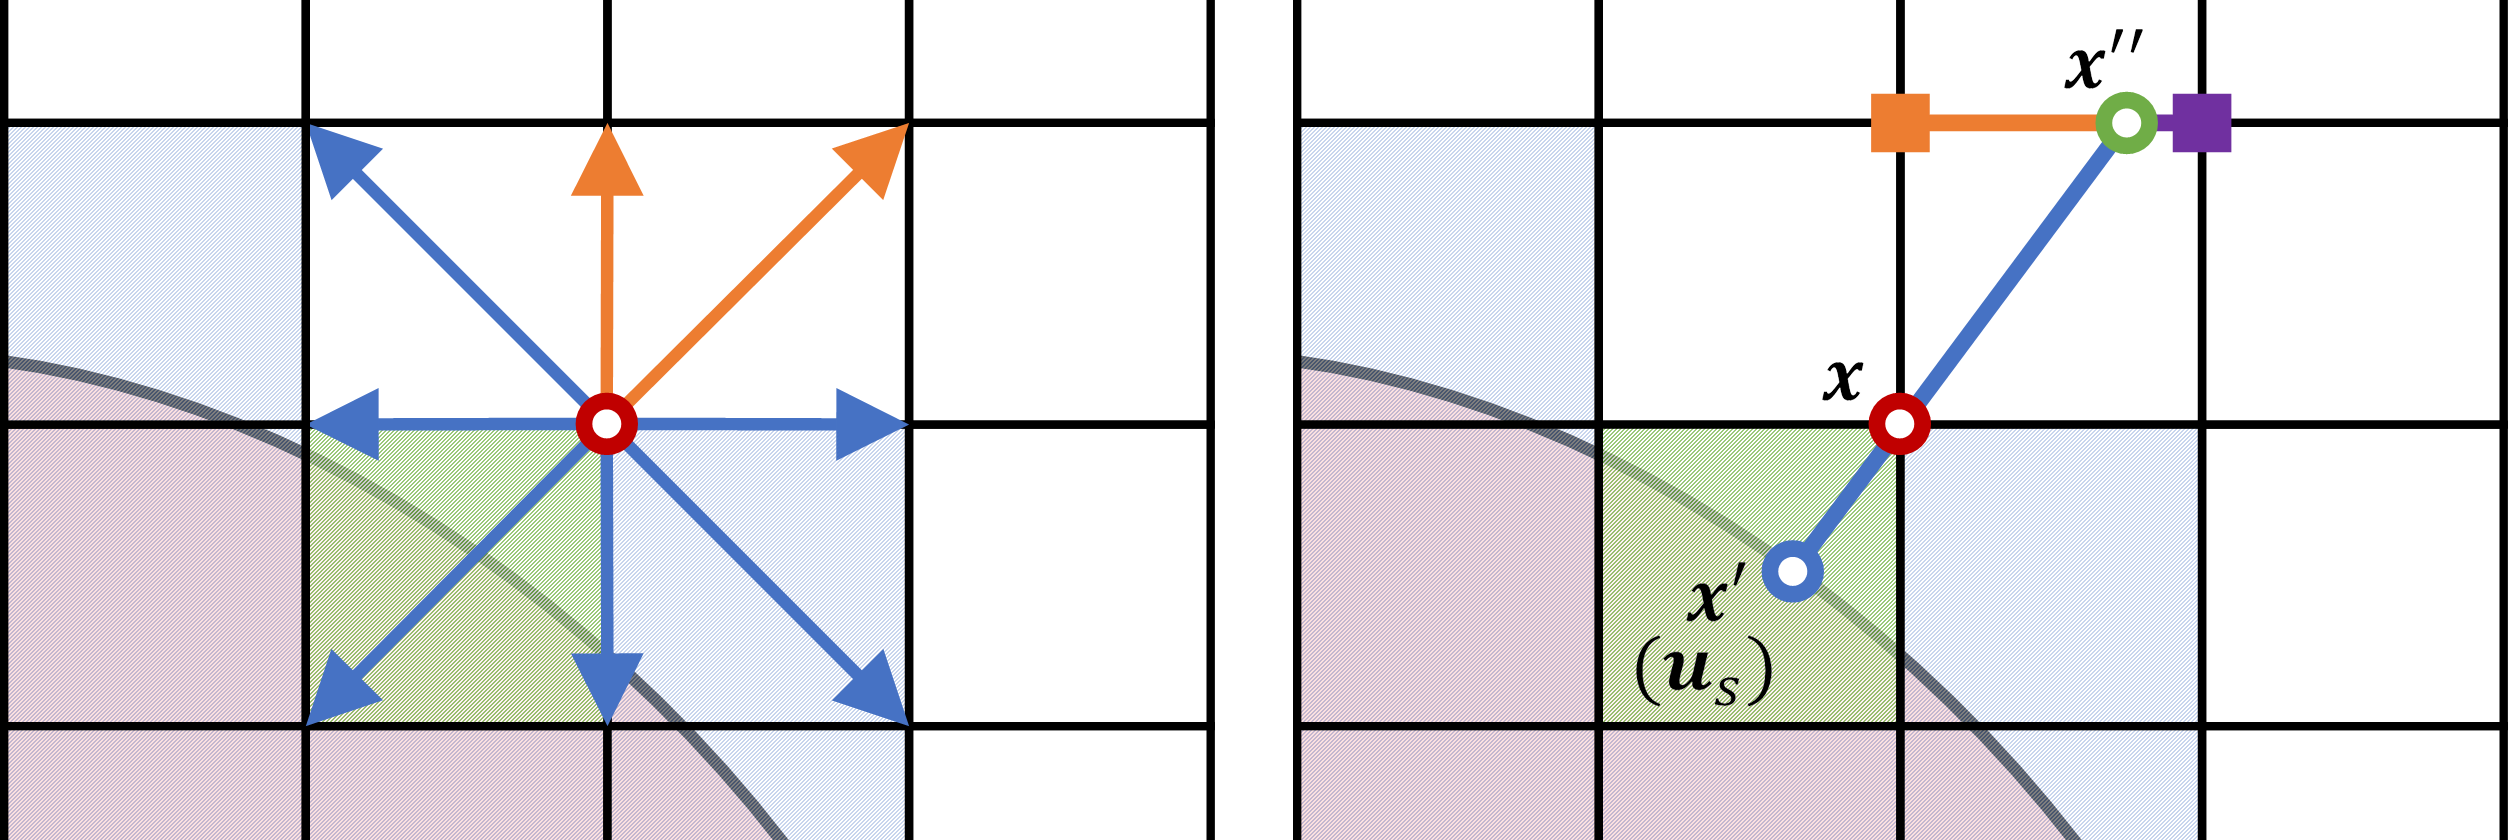
\includegraphics[width=0.95\columnwidth]{figures/cutcell_and_interpolation.png}
    \bicaption{切削网格中的速度插值。左图:因为固体边界存在而产生的切削网格 (图中标为绿色)。右图:流体中的切削网格格点$\bm{x}$ (图中标为红色圆圈) 的速度,需要通过固体边界的投影点$\bm{x}{'}$ (图中标为蓝色圆圈),与该投影点到格点的延长线与下一个网格的交点$\bm{x}{''}$ (图中标为绿色圆圈) 进行速度的线性插值得到。}{Interpolation of velocity on cut-cell nodes. Left: cut-cell (marked in green) intersecting a solid boundary; Right: the velocity on a cut-cell node $\bm{x}$ inside the fluid region (red circle) needs to be interpolated using the velocities of its projected point $\bm{x}{'}$ onto the solid boundary (blue circle) and the intersected point between the ray from the projected point to the cut-cell node and the interpolated fluid point $\bm{x}{''}$ (green circle), where the velocity can be reliably evaluated through simple linear interpolation.}
    \label{img:cutcell_and_interpolation}
\end{figure}

\begin{figure}[htb]
    \centering
      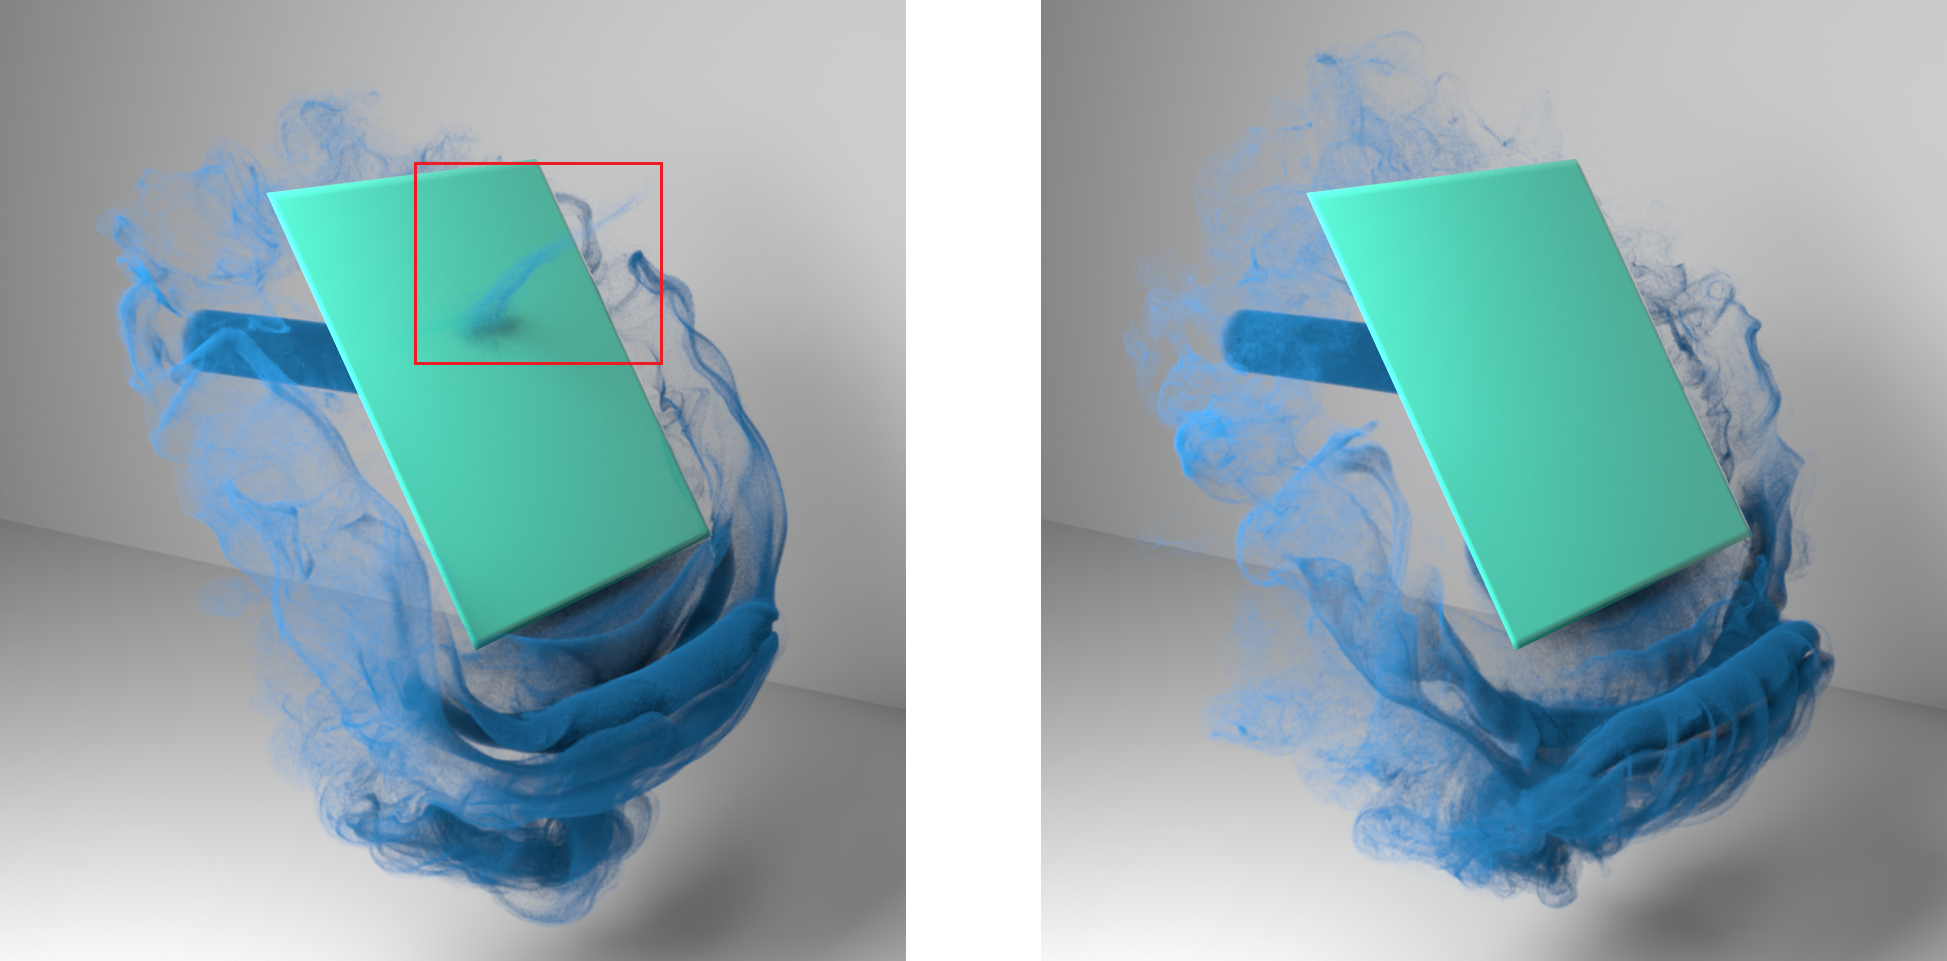
\includegraphics[width=0.97\columnwidth]{figures/comparison_with_ib.png}
    \bicaption{浸没边界法造成的泄露。当有薄板存在时,Li等~(\citeyear{Li-2020}) 所使用的浸没边界法 (左图) 与我们的方法的对比 (右图)。因为惩罚力会分布到薄板两侧,扩散边界浸没边界法可能会产生泄露 (见图中红色方框),而我们的方法可防止此现象。}{Leakage of immersed boundary. For a kinetic fluid simulation coupled with a thin plate, the immersed boundary method used by Li et al.~(\citeyear{Li-2020}) (left) is compared with our method (right). Due to force spreading in both sides of the thin plate, this recent coupling approach employing a diffuse-interface immersed boundary method may generate leakage through the plate (see red box), while our method prevents this issue by design.}
    \label{img:comparison_with_ib}
\end{figure}

\begin{figure}[htb]
    \centering
      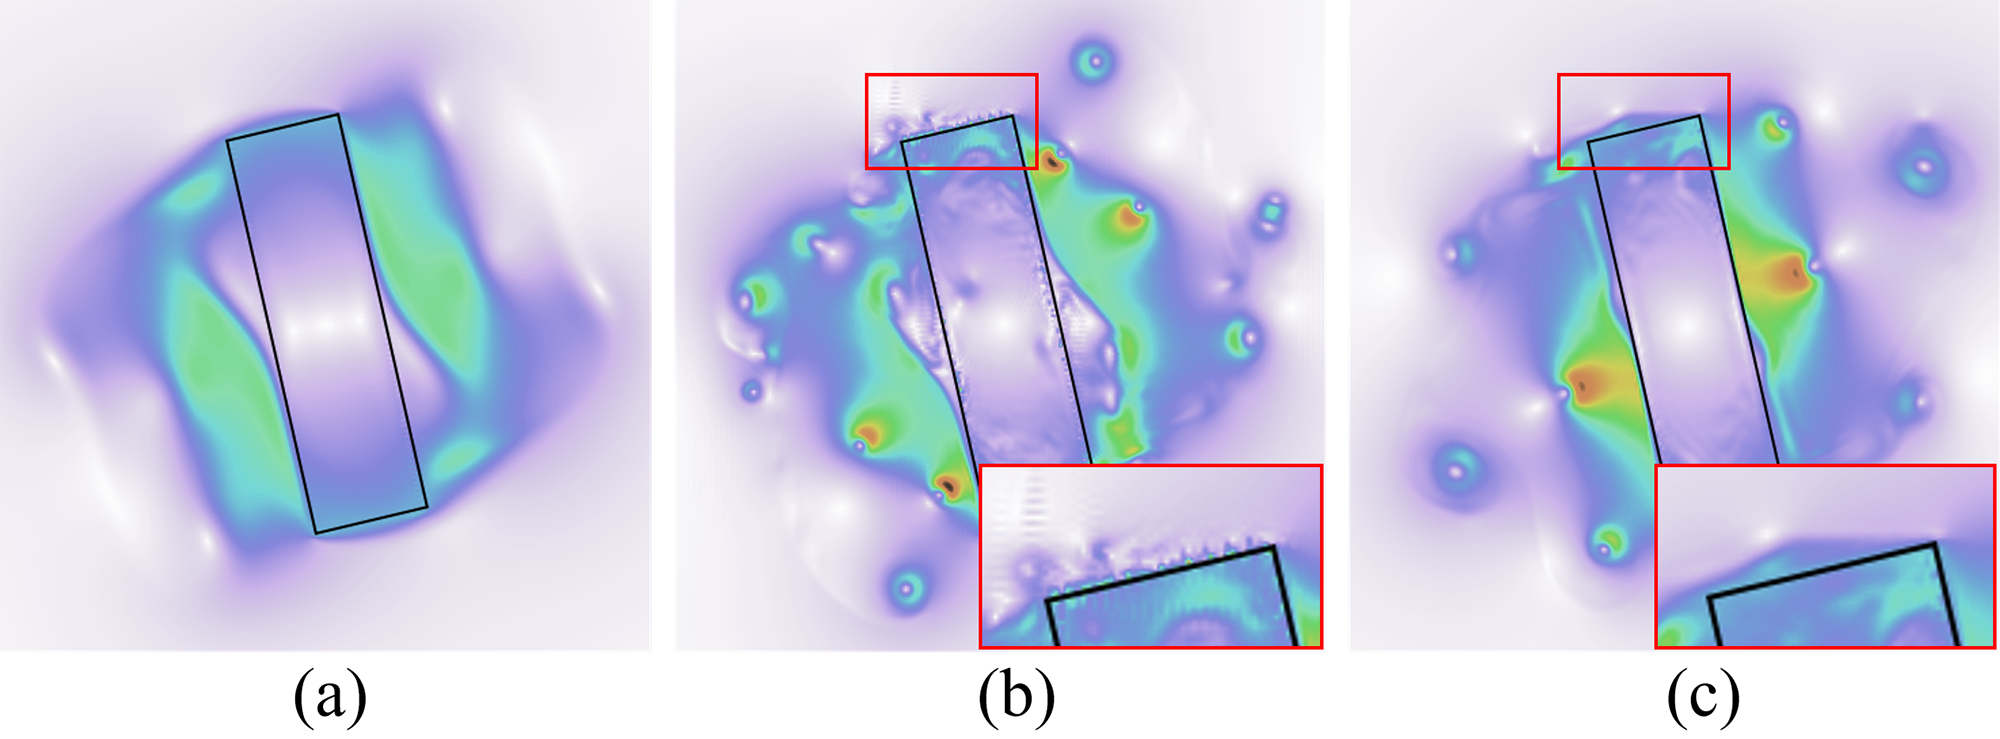
\includegraphics[width=0.95\columnwidth]{figures/ib-mbb.png}
    \bicaption{不同雷诺数下的简单反弹边界处理方法。(a) 在低雷诺数下,简单反弹边界没有造成视觉不正确的现象;(b) 但在高雷诺数下,固体边界会有很强的锯齿现象,从而对稳定性有较大影响;(c) 我们的方法在与 (b) 同样的高雷诺数情况下看不到视觉不正确的现象。}{Simple bounce-back under different Reynolds numbers. (a) a plain simple bounce-back scheme generates no visual artifacts for  flows with low Reynolds number; (b) however, it exhibits strong aliasing artifacts near the solid boundary for high Reynolds number flows, which may seriously influence stability; (c) our new boundary treatment for the same high Reynolds number as in (b) is artifact-free, generating the type of vortices expected from such an example.}
    \label{img:Immersed_Bounce_back}
\end{figure}

% Sec 3.2
\section{方法}
我们的混合方法主要包含下面三个部分:
\begin{itemize}
\item 双面简单反弹边界:我们首先介绍一个简单反弹边界方法的变种,即切削网格边界的两侧都会发生分布函数的反弹,而不只在一侧发生,从而不再需要追踪格子随物体运动的状态变化;
\item 切削网格的速度修正:我们通过在切削网格内进行单边的速度修正,大幅提升仿真的稳定性,同时压制边界上的速度误差;
\item 固体受力:最后我们通过介观与宏观的混合,求出流体转移至固体的动量,从而获得固体受力以驱动固体运动。
\end{itemize}

我们将在下面依次介绍这三部分内容。

\subsection{双面简单反弹边界}
在第~\ref{sec:boundary_treatment} 节中,我们回顾了简单反弹边界方法。一般来说,反弹边界都只应用于流体点。然而随着物体的运动,流体点可能被固体覆盖成为固体点,固体点也可能重新变为流体点。这个转换过程不止需要追踪格点状态,并且需要进行速度的插值,甚至外插。这样会在高雷诺数下在固体边界上产生很强的耗散误差。为了避免这一现象,我们对所有切削网格内的点都进行分布函数反弹,而不只针对流体点。我们称该方法为\emph{双面简单反弹边界方法}。该方法依旧可以避免流体泄露,即使有亚网格物体存在。但这并没有改善固体边界的速度锯齿现象与大速度梯度造成的误差,所以我们引入下一节中介绍的速度修正方法。

\subsection{切削网格的速度修正}
因为我们谋求的是低阶 (线性) 精度的边界处理,我们提出在双面简单反弹边界之后,通过沿固体边界的法向方向对速度线性插值,来对速度场进行修正。修正的方式为对流场施加惩罚力。更具体地说,我们先通过切削网格点周围的固体和流体速度插值,得到一个切削网格点上的期望速度。之后通过当前速度与期望速度的差计算惩罚力,从而修正速度场。

\paragraph{切削网格点上的期望速度}
切削网格点上的期望速度可通过其邻近的可靠速度插值得来。对于处于固体内部的切削网格点,它们的期望速度必须与那一点的固体速度一致,这个速度可以通过固体的运动状态直接获得。
对于流体中的切削网格点,我们通过一个线性插值,获得其期望速度。该插值方法如图~\ref{img:cutcell_and_interpolation} 中右图所示。对于切削网格点$\bm{x}$点,我们首先计算它在固体边界的投影点位置$\bm{x}'$,之后从$\bm{x}'$向$\bm{x}$打一条射线,该射线与下一个网格面的交点为$\bm{x}''$。如果这个面上的所有点都不是切削网格点,$\bm{x}''$点的速度就可以通过该面上的点线性插值得来 (二维中是线性插值,三维中是双线性插值)。如果这个面上存在点是切削网格点,则可寻找下一个交点,直到找到满足条件的交点。此时$\bm{x}$点的期望速度则可通过线性插值得到:
\begin{equation}  \label{eq:vel_lerp}
\hat{\bm{u}}(\bm{x})=(1-\alpha)\bm{u}_s + \alpha \bm{u}(\bm{x}'')\;,
\end{equation}
其中$\alpha=\|\bm{x}-\bm{x}'\|/\|\bm{x}''-\bm{x}'\|$,$\bm{u}_s$是固体边界上投影点$\bm{x}'$的速度。

\paragraph{基于惩罚力的速度修正}
由于切削网格点$\bm{x}$上的期望速度$\hat{\bm{u}}(\bm{x})$可能与分布函数反弹后的宏观速度$\bm{u}(\bm{x})$有偏差,我们构造如下的惩罚力$\bm{F}_p(\bm{x})$
\begin{equation} \label{eq:penaltyForce}
\bm{F}_p(\bm{x}) = \hat{\bm{u}}(\bm{x})-\bm{u}(\bm{x})\;,
\end{equation}
施加在点$\bm{x}$上,做法与Li等~(\citeyear{Li-2020}) 中相同。我们将惩罚力投影至分布函数空间,分布函数使用最高阶的埃尔米特多项式展开,以维持精度与稳定性。由于反弹边界已经承担了大部分的边界处理,这里的惩罚力会比传统浸没边界法中的惩罚力小很多,只作为一个速度的修正出现,于是我们也不需要采用Li等~(\citeyear{Li-2020}) 中的时间重缩放来缩短物理时间步长从而提升稳定性。这可以使仿真效率进一步提升。

\begin{figure}[htb]
    \centering
      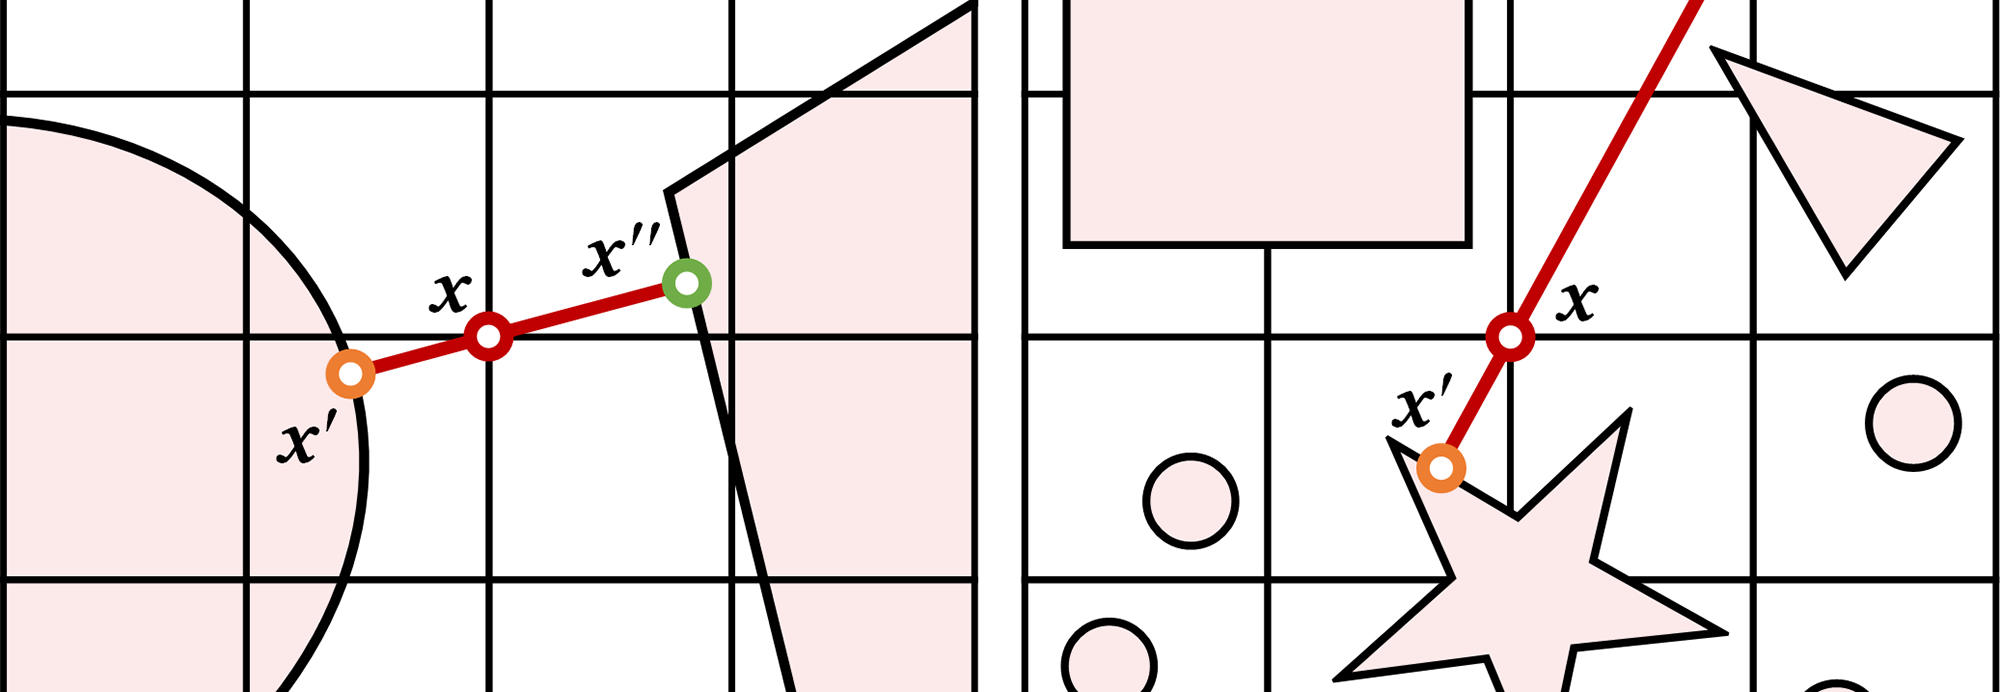
\includegraphics[width=0.95\columnwidth]{figures/cutcell_special_cases.png}
    \bicaption{两种邻近物体的情况。左图:从固体边界点$\bm{x}'$起始的射线经过$\bm{x}$点,在交到网格面之前,便相交于另一个物体上。这种情况,$\bm{x}''$是另一个固体边界点。右图:一个切削网格点可能完全被切削网格面包围,所以找不到任何非切削网格面。}{Two cases of solid proximity. Left: the ray starting from a boundary point $\bm{x}'$ through a grid node $\bm{x}$ may hit another boundary surface point before it intersects with the non-cut-cell face; in this case, $\bm{x}''$ locates at another boundary point. Right: a cut-cell node may be surrounded by all cut-cell faces, so a ray may not hit any non-cut-cell face nearby.}
    \label{img:handling_proximity}
\end{figure}

\paragraph{一些特殊情况}
当流体中的物体间距离接近网格尺度的时候,有时$\bm{x}''$的速度会无法从周围的非切削网格点插值得到。一种情况是从$\bm{x}'$点射出的射线在交到网格面之前,便相交于另一个物体上 (图~\ref{img:handling_proximity} 中左图)。那么由于这个交点的速度是已知的,我们可以用这一速度替代先前提到的非切削网格点的速度。另一种情况是,因为物体之间过于接近,射线无法找到任何非切削网格面。这个时候我们只得抛弃速度修正过程,而只采用双面简单反弹边界作为边界处理。

\begin{figure}[htb]
  \centering
    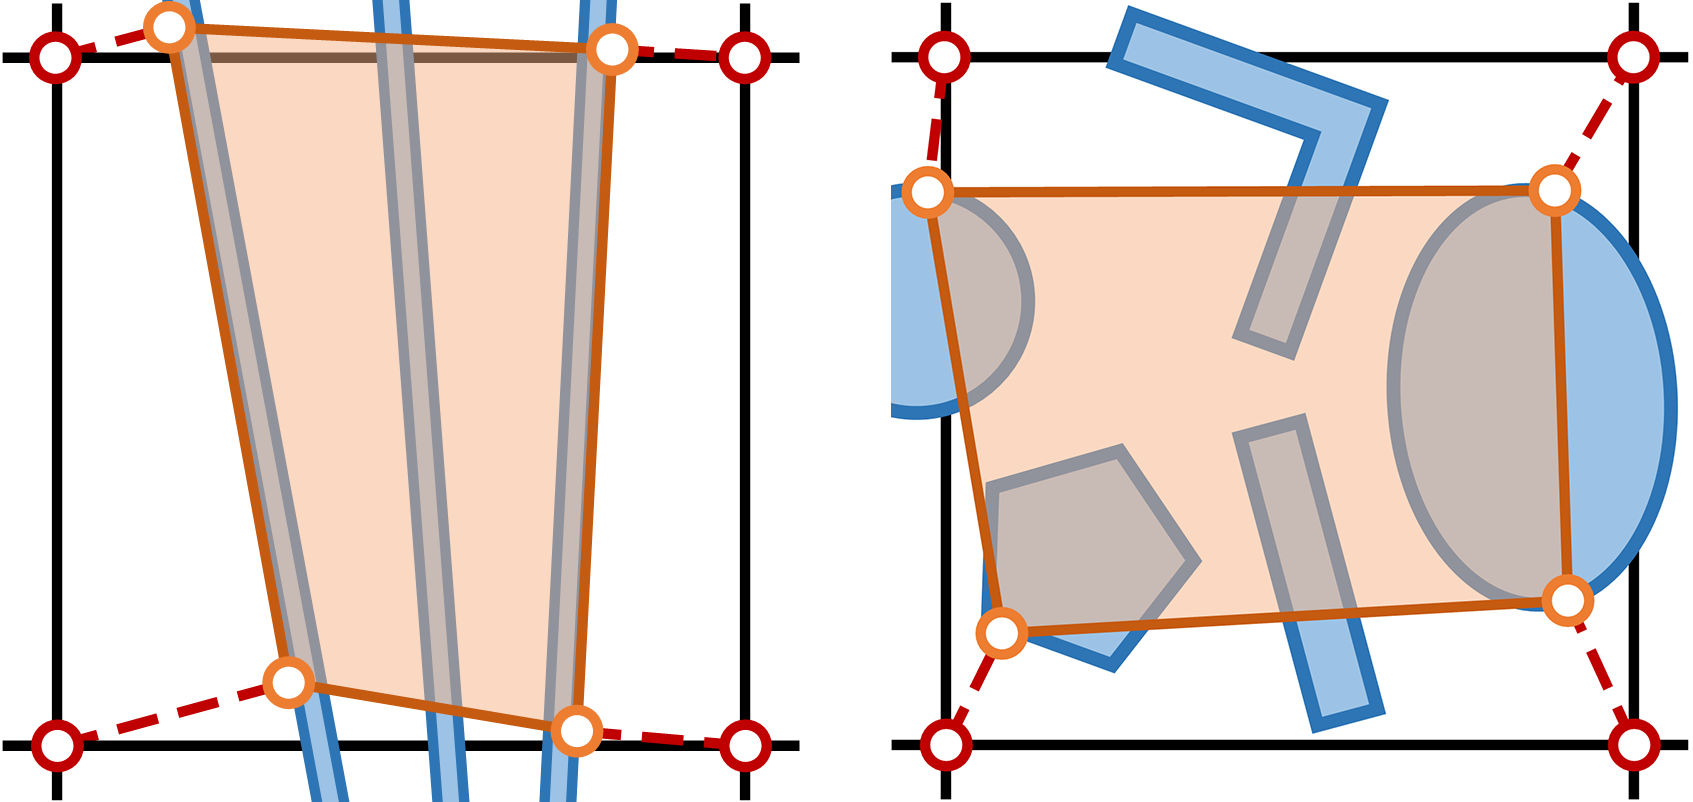
\includegraphics[width=0.9\columnwidth]{figures/sub_grid_approximation.png}
  \bicaption{亚网格近似。在亚网格物体存在时,我们将每个切削网格点投影至其最近的边界采样点。这等同于使用一个包围体积 (橘色区域) 来近似一个网格中的多个亚网格物体。}{Sub-grid approximation. To handle sub-grid scale solid structures, we project each cut-cell node onto its nearest boundary sample point. This basically amounts to using bounding volumes (orange regions) to approximate multiple thin structures within a cut-cell.}
  \label{img:sub_grid_approximation}
\end{figure}

\paragraph{亚网格近似}
当数量众多的薄板或细棒存在时,有可能一个流体网格中会包含多个这样的物体,尤其在网格较粗的情况中 (见图~\ref{img:sub_grid_approximation} ),此时边界的精度是无法保证的。此时,我们使用一个包围体积,来近似这些存在于一个网格中的多个物体。所以我们依然可以将流体点投影至距离最近的固体边界点来计算惩罚力。

\paragraph{讨论}
我们的惩罚力修正是基于法向方向的线性速度插值。这个修正可被认为是一个滤波器,来压制在高雷诺数下,简单反弹边界造成的固体边界周围的速度震荡。这个修正可以有效地提升在湍流流固耦合仿真的稳定性,使得我们在相对粗糙的网格中也能获得视觉上可信的仿真结果。然而,这依然只是一个一阶的线性修正,所以要获得高物理精度的仿真需要高分辨率网格作为基础。但考虑到我们主要面向图形学应用,我们不考虑在构造更加复杂的速度修正方法。

\subsection{固体受力}
因为要做到流固的双向耦合,我们需要讨论流体中固体的受力,也即流体传递给固体的动量。我们在边界中使用了反弹边界与速度修正的结合,所以我们在讨论固体受力时也分为两部分来讨论。我们首先讨论双面反弹边界对固体受力的贡献。在双面反弹边界之后,我们先将由公式~\ref{eq:bounce-back} 带来的动量交换进行累计。更具体地说,迁移过程后,$t$时刻$\bm{x}$点的动量可以表达为
\begin{equation}
  \bm{p}(\bm{x}) = \sum_{i}\bm{c}_if^*_i(\bm{x},t).
\end{equation}
如果$L$是$\bm{x}$点切削速度方向的集合 (即与固体边界相交的速度方向),每一个$L$中的速度方向都会发生分布函数反弹,那么$\bm{c}_j$方向的流固动量交换是
\begin{equation}
  \smash{-\bm{c}_{j}\,(f^*_{j}(\bm{x}) + f^*_{j'}(\bm{x}))}.
\end{equation}
从而,在$\bm{x}$点交换的动量和$\Delta \bm{p}$为
\begin{equation}
\Delta \bm{p}(\bm{x})= - \sum_{j\in L} \bm{c}_{j}\,(f^*_{j}(\bm{x}) + f^*_{j'}(\bm{x})),
\end{equation}
其中我们不将$(\Delta x)^3$显式写出 ($\Delta x$是网格大小),因为在正则化LBE空间中这一项为1。
那么反弹边界部分所贡献的固体受力是所有点动量交换的和,即
\begin{equation}
\bm{F}_{B}\equiv \sum_{\bm{x}} \Delta \bm{p}(\bm{x}),
\end{equation}
其中除以$\Delta t$ (时间步长) 也被隐去,因为其在正则化LBE空间中也为1。类似地,我们可以获得总的力矩
\begin{equation}
\bm{\tau}_{B}\equiv \sum_{\bm{x}} (\bm{x}-\bm{x}_{C})\times\Delta \bm{p}(\bm{x}),
\end{equation}
其中$\bm{x}_{C}$是物体质心的位置。

接下来我们继续讨论速度修正对固体受力的贡献。我们认为这个速度修正的来源依旧是固体的存在,所以这个力的来源是固体本身。那么固体理应受到一个与惩罚力大小相同,方向相反的反作用力。那么这一部分固体所受到的合力$\bm{F}_{C}$与合力矩$\bm{\tau}_{C}$可以表达为
\begin{equation}
\bm{F}_{C} = - \sum_{\bm{x}}\bm{F}_p(\bm{x}), \quad \bm{\tau}_{C} = - \sum_{\bm{x}} (\bm{x}-\bm{x}_{C})\times\bm{F}_p(\bm{x}).
\end{equation}

所以固体受到的合力$\bm{F}_s$与合力矩$\bm{\tau}_s$是上述两部分贡献的和:
\begin{equation}
\bm{F}_s = \bm{F}_{B} + \bm{F}_{C} \text{ and } \bm{\tau}_s = \bm{\tau}_{B} + \bm{\tau}_{C}.
\end{equation}

\section{算法优化}
\subsection{几何近似}
我们的混合边界处理中需要许多的几何计算,如将流体点投影至固体表面,或将速度方向与固体边界进行求交等。我们还需要识别切削网格点,以及它们的状态 (属于流体区域或固体区域)。许多工作阐述了如何准确地进行这样的几何计算~\cite{Azevedo-2016,Robinson:2009}。但由于固体边界的形状可能十分复杂,这一过程可能非常耗时,不利于维持LBM高并行度的优势。
为了在效率与精度间取得平衡,我们提出一系列的几何近似计算方法,以在不影响视觉可信度的情况下提升计算效率。

\begin{figure}[htb]
  \centering
    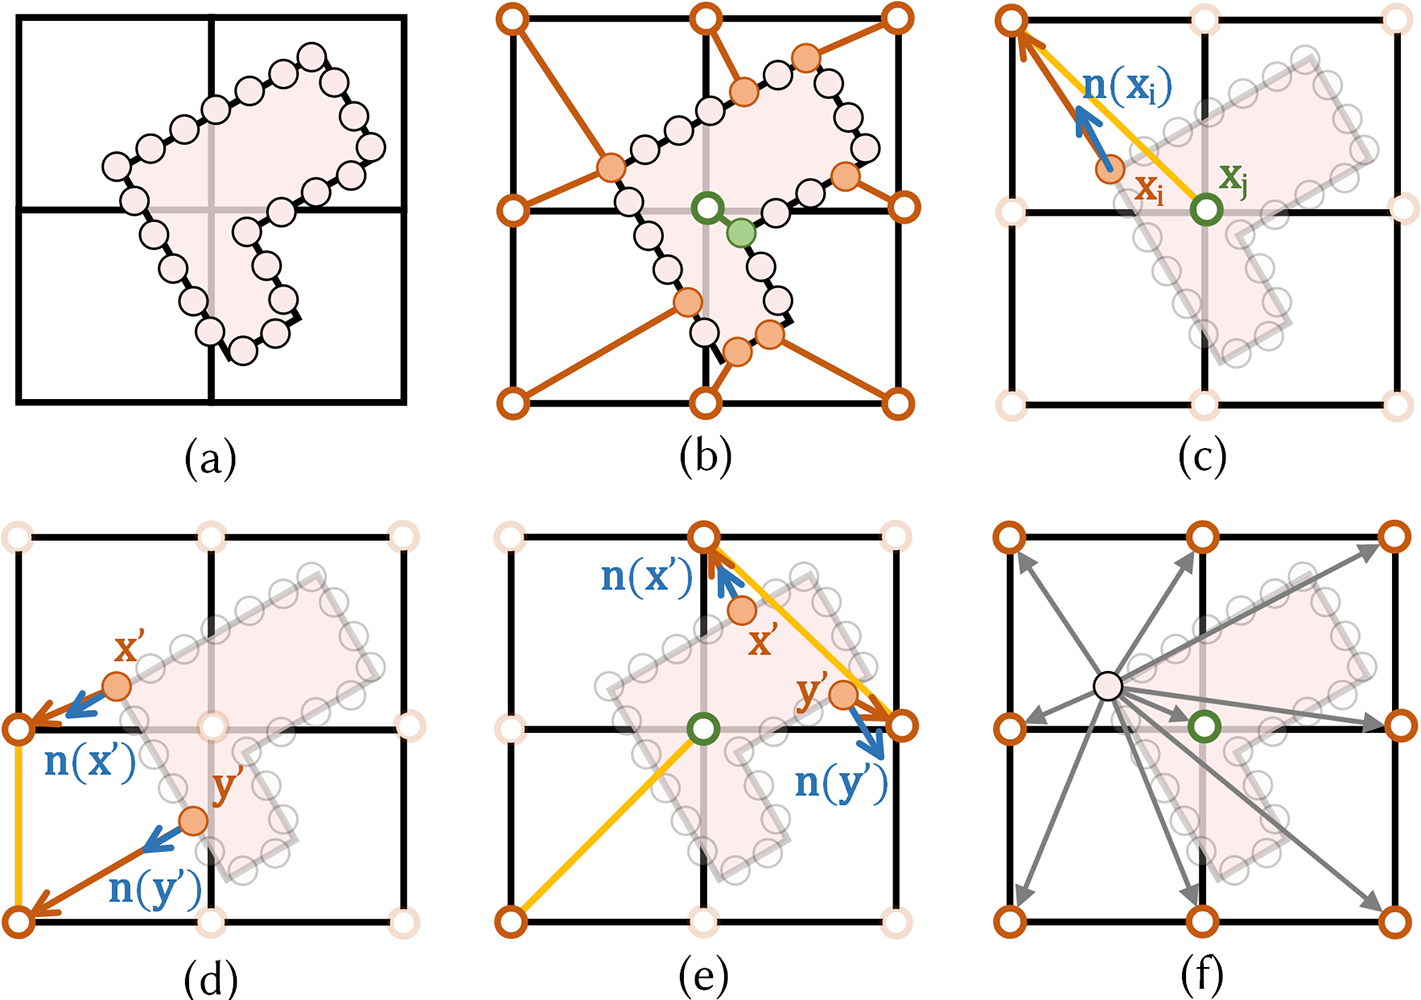
\includegraphics[width=0.97\columnwidth]{figures/geometric_computing.png}
  \bicaption{高效几何近似计算。对于一个固体,我们首先对它的边界采样 (a),然后切削网格点的投影点可以被近似为距其最近的采样点 (b)。为了检验某个速度方向 (图中标为黄色) 是否与固体边界相交,我们可以检查这个方向的两端是否有固体点存在。如果一端是固体点另一端是流体点,则我们认为其跨过了固体边界 (c) (图中绿色点为固体点,橘色点为流体点)。对于两端都是流体点的情况,我们检查这两个流体点投影点的法向,如果它们有类似的朝向 (d) 则认为该方向没有跨过边界,相反则认为其跨过边界 (e)。在GPU实现时,我们从所有的固体采样点出发,令每个固体采样点寻找其周围的流体切削网格点,而不是从流体点出发。}{Efficient geometric approximation. Given a solid geometry, we first sample its boundary (a); then the projected points of cut-cell nodes can be simply approximated by the nearest sample (b). To examine whether a link (yellow) crosses the solid boundary, we first check if solid nodes are involved. If the ends of the link are fluid and solid nodes, then it crosses the solid boundary (c) (green cut-cell nodes are inside the solid, whereas orange ones are in the fluid). For links connecting fluid nodes, we check the normals of the two projected cut-cell nodes forming the link; if the two normals have the same orientation (d), the link does not cross the solid boundary; otherwise, it intersects the solid boundary (e). For GPU implementation, we parallelize over solid samples instead of cut-cell nodes, where each solid sample will check its surrounding region of cut-cell nodes.}
  \label{img:geometric-computing}
\end{figure}

\paragraph{表面采样与切削网格识别}
为了加速计算,我们可以使用采样点而不是实际的几何来表达边界。这一过程需要对固体表面进行均匀采样,如使用泊松圆盘采样 (Poisson-disk Sampling)~\cite{dunbar2006spatial}。注意这也要求固体模型应该是密封的。每一个采样点$\bm{x}_s$在采样时可获得一个由边界朝外的法向$\bm{n}(\bm{x}_s)$。之后如果有网格中包含至少一个边界采样点,这个网格就可以被识别为切削网格 (如图~\ref{img:geometric-computing} (a))。

\paragraph{高效切削网格投影}
在几何计算中一个最重要的 (也可能是最耗时的) 部分是将流体点$\bm{x}$投影至固体表面上,以得到投影点位置$\bm{x}'$。传统方法可能会构建一个树形结构,然后搜索距离$\bm{x}$点最近的三角形~\cite{wang-2012}。在这里我们使用一个高效的近似算法来替代这一过程,我们在固体表面选择一个距离$\bm{x}$点最近的采样点$\bm{x}_s$,并满足
\begin{equation}\label{eq:is_in_fluid}
(\bm{x}-\bm{x}_s)\cdot \bm{n}(\bm{x}_s) \geq 0\;
\end{equation}
来近似采样点$\bm{x}'$。公式~\ref{eq:is_in_fluid} 这个约束可以避免我们选择到错误朝向的采样点。如果没有满足这个约束的采样点,那么这个点应该被标记为固体点 (如图~\ref{img:geometric-computing} (b))。这个基于采样点的技术可以达到很高的并行度,但精度很显然依赖于采样密度。所以在实现中,我们需要保证每个切削网格内有足够的采样点数。一般我们设置泊松圆盘采样的采样距离不超过网格大小的一半。

\paragraph{近似反弹边界处理}
在双面反弹边界处理中,我们必须要识别出与固体边界相交的速度方向 (见图~\ref{img:bounce_back_scheme} )。对于厚物体,由于我们已经对切削网格点属于流体点或固体点有所标记,我们只许对速度方向的两端点的状态进行识别。如果两个端点分别为流体点和固体点,则这个速度方向与固体边界有相交。但是对于薄物体,可能存在两端均是流体点,但依然与固体表面相交的情况。所以我们要进行特殊识别。
对于从$\bm{x}$至$\bm{y}$点的速度方向,我们检查这两个点的投影点$\bm{x}'$与$\bm{y}'$的法向朝向是否不一致,即$\bm{n}(\bm{x}')\!\cdot\!\bm{n}(\bm{y'})\!<\!0$ (如图~\ref{img:geometric-computing} (d)与(e))。
如果朝向不一致 (图~\ref{img:geometric-computing} (e) 即为此情况),则我们认为$\bm{x}$点与$\bm{y}$点处于边界的不同侧,所以这个速度方向是与固体表面相交的。则我们应在这个方向上进行反弹边界处理。

\subsection{GPU实现}
% All of our algorithms so far, including geometric approximations, are designed to involve \emph{purely local computations} with relatively simple algebra. It results in an overall coupling approach that is straightforward to implement on a parallel computing platform such as a GPU for efficient simulation: it respects the embarrassingly parallel nature of LBM. Our simulation method is very scalable since it can run on either a single or multiple GPU(s) by leveraging the GPU optimization techniques presented in \cite{Chen-2021}; our examples are computed with only one GPU, except for a high-resolution simulation shown in Fig.~\ref{fig:result-city} where we used two GPUs instead. We discuss next a few specific accelerations and optimizations we incorporated in our GPU implementation in order to improve the overall performance for our two-way coupled simulations. \vspace*{-1mm}

% \paragraph{Memory layout}
% For LBM, a structure-of-arrays (SoA) memory layout is recommended to store discrete distribution functions $f_i$ of all grid nodes to improve cache utilization and thus improve performance~\cite{Chen-2021}. We follow this recommendation in our GPU implementation as our tests showed that the SoA layout is still the most efficient, even with our new coupling strategy. \vspace*{-1.5mm}

% \paragraph{Efficient collision evaluation}
% Also discussed and demonstrated in~\cite{Chen-2021} was the computation of the inverse of the central-moment projection matrix $\bm{M}(\bm{u})$. They argued that this inverse should be computed analytically to preserve accuracy, but the algebraic expression is very lengthy and occupies many registers, resulting in low achieved GPU occupancy in practice.
% However, we observed that if one performs an analytical LU decomposition~\cite{fei2018three} of $\bm{M}(\bm{u})^{-1}$, many elements of the resulting triangular matrices are very close to zero. Thus, we can discard those close-to-zero elements and employ the usual sparse matrix format to store the decomposed matrices, decreasing drastically the terms needed to compute the inverse. This does not influence accuracy (the reconstruction error is below machine accuracy), but significantly reduces the use of registers; the performance for parallel collision calculation is then three times faster on average compared to the implementation using~\cite{Chen-2021} on the same GPU. \vspace*{-1.5mm}

% \paragraph{Parallel cut-cell point projection and identification}
% Throughout all the stages of our hybrid coupling algorithm, a key operation is to project a cut-cell node onto the nearest solid boundary, which is approximated by searching for the nearest sample point on the solid boundaries.
% While there are traditional
% GPU implementations to achieve this task in parallel over cut-cell nodes, they often generate load imbalance and low GPU occupancy issues.
% %as pointed out in~\cite{Chen-2021} for their case of a GPU-based immersed boundary method.
% Thus, as suggested in \cite{Chen-2021}, we parallelize over solid samples instead --- but proceed differently to improve performance.
% For each sample, we compute the distance to each node of the cut cell in which the sample is located (see Fig.~\ref{fig:geometric-computing} (f)) and compare with the distance stored in that node: if the distance of the sample to a cut-cell node is smaller than the current distance stored in that node, we update this distance with the new distance, and change the index of the solid sample stored along with that same node.
% Since the same cut-cell node may be accessed from multiple solid sample threads, we employ an atomic comparison operation to avoid thread conflicts.
% Note that Eq.~\eqref{eq:is_in_fluid} still needs to be satisfied for every comparison, so the identification of solid nodes is included in the process.

\section{对比与仿真结果}
\subsection{对比}
此节中我们将我们的方法与图形学中近期提出的LBM仿真方法~\cite{Li-2020} 进行定量与定性的对比,包括与实际实验的对比。我们还针对计算效率,讨论基于Li等~\citeyear{Li-2020} 的性能改进~\cite{Chen-2021} 与我们方法的比较。

% \paragraph{与图形学中现有方法的对比}
% Recently, a kinetic solver demonstrated strong capabilities for fluid-solid two-way coupling with turbulent flows, employing a DI-IB method to treat solid boundaries~\cite{Li-2020}.
% However, many limitations were acknowledged.
% Since DI-IB method does not act in a one-sided manner, it exhibits flow penetration for obstacles of size equal or smaller than a grid cell.
% Fig.~\ref{fig:comparison_with_ib} shows a comparison for a 3D jet flow shot onto a thin plate, where (a) \cite{Li-2020} creates an unexpected smoke flow on the other side of the plate as marked by the red box, while (b) our new method correctly enforces non-penetration through this thin structure.
% Additionally, the low accuracy of the DI-IB method can fail to produce the right simulation result, especially for boundary layers around a solid object when the flow is turbulent.
% %as a consequence, Li et al.~\shortcite{Li-2020} can in fact produce inaccurate qualitative results.
% A clear and obvious example of this issue is the airflow simulation around a moving car model shown in Fig.~\ref{fig:comparsion_car_ib_ours}. As is well-known by car designers, a reasonable design for a car should induce a flow separation at the rear of the car to reduce aerodynamic drag, and the use of rear spoilers (or ``ducktails'') helps push the flow separation further away, as can be seen in Fig.~\ref{fig:comparsion_car_design} (d) in a real wind tunnel experiment. The DI-IB method of \cite{Li-2020} in this case predicts a boundary layer which separates at the top of the car, far too forward compared to the wind tunnel experiment; instead, our new boundary treatment method (for exactly the same grid resolution) reproduces the correct behavior.
% To demonstrate further how a small, thin structure like a ducktail can affect the flow around a car, we also show in Fig.~\ref{fig:comparsion_car_design} that the absence of the rear spoiler changes dramatically the turbulence patterns witnessed behind the car: the spoiler thus acts as a wake generator, and sometimes lift reducer as well, to improve the maneuverability at high speed. These two examples both point to our method having an improved accuracy compared to the existing LBM methods in graphics.\vspace*{-1mm}

\begin{figure}[htb]
  \centering
    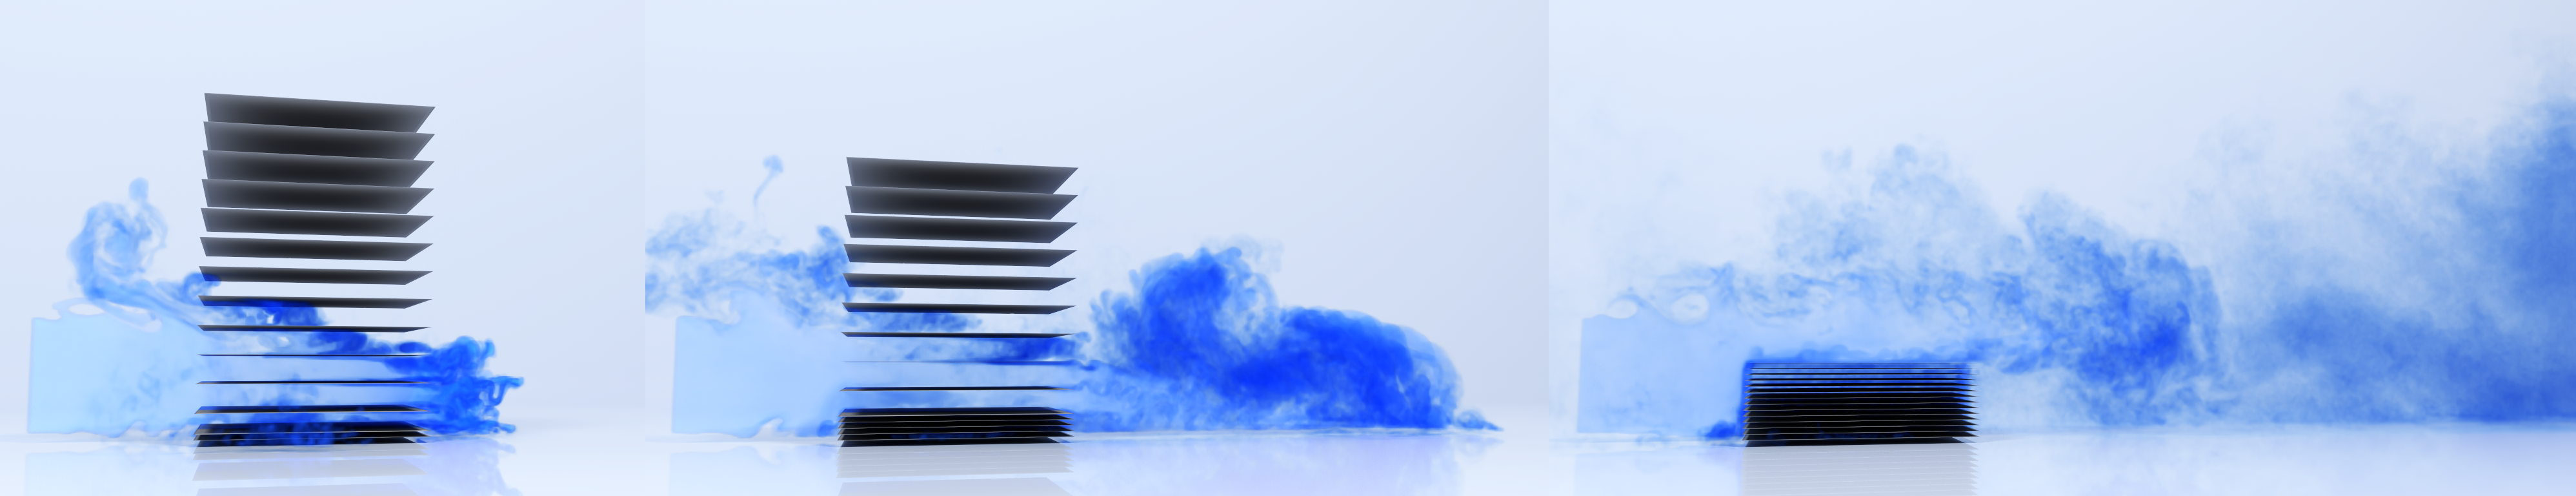
\includegraphics[width=0.99\columnwidth]{figures/result_thin_shell_sub_grid.png}
  \bicaption{烟雾经过层叠的板子。烟雾吹过一系列下落的薄板。虽然薄板在分开时烟雾可以通过,当它们层叠在一起时却形成一个密闭的障碍物。我们边界处理中的亚网格近似可以同时处理这两种不同情况,当板子加速靠近时,中间的流体会被加速,而它们紧贴时会成为一个厚的物体。}{Smoke flow through stacked plates. Smoke is blown towards a falling stack of thin plates. While smoke freely flows between separate plates, they become an airtight obstacle when they are stacked on top of each other. Our boundary treatment based on subgrid approximation deals with both cases seamlessly: plates getting closer accelerate the flow in between them, while tightly stacked plates are treated as thick solids.}
  \label{img:result-thin-shell-sub-grid}
\end{figure}

\begin{figure}[htb]
  \centering
    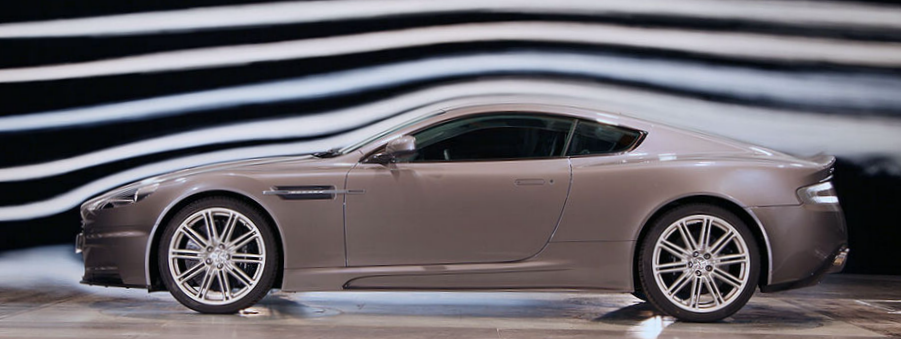
\includegraphics[width=0.99\columnwidth]{figures/car_wind_tunnel.png}
  \bicaption{车的风洞测试。车周围的气流可视化展示了车身的设计使得气流直到后备箱才发生边界层分离,这样可以有效减少风阻与震动。图片版权来自\textit{Auto Motor und Sport}, \copyright Frank Herzog/Sportauto.}{Wind-tunnel test of a car. A wind tunnel visualization of the airflow around a car shows that the design of the body delays boundary layer separation until the trunk, which reduces drag and vibration in practice. Image courtesy of \textit{Auto Motor und Sport}, \copyright Frank Herzog/Sportauto.}
  \label{img:car_wind_tunnel}
\end{figure}

\begin{figure}[htb]
  \centering
    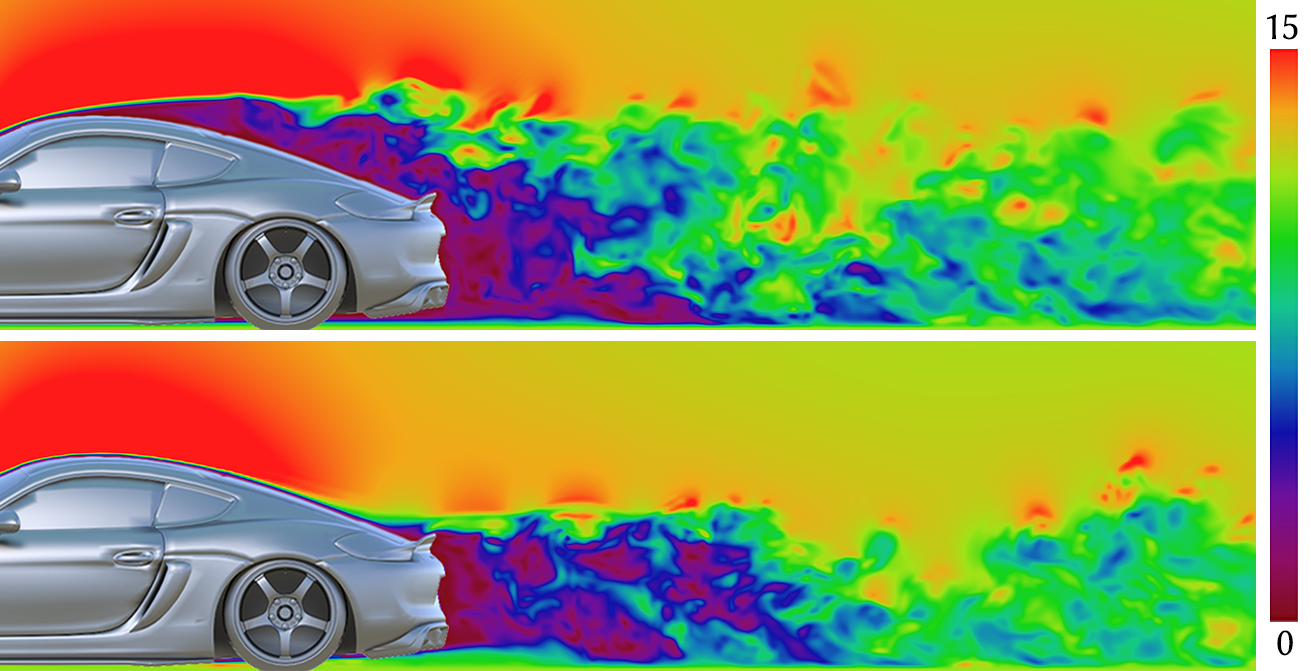
\includegraphics[width=0.99\columnwidth]{figures/comparsion_car_ib_ours.png}
  \bicaption{DI-IBM~\cite{Li-2020} (顶图) 与我们的方法 (底图) 进行气动仿真的对比,速度场截面使用颜色可视化 (单位为$km/h$)。我们的仿真更贴近图~\ref{img:car_wind_tunnel} 中风洞的实际实验,而DI-IBM在车顶即开始发生边界层分离,不切合实际情况。}{Comparison of aerodynamic simulations. DI-IB method~\cite{Li-2020} (top) vs. our result (bottom), using a visualization showing the color-coded velocity field magnitude (in $km/h$) of a cross section. While our simulation matches the wind-tunnel visualization of air flow around a car as Fig.~\ref{img:car_wind_tunnel} demonstrates, the DI-IB method, on the other hand, fails to have accurate boundary treatment, leading to unreasonable boundary layer separation at the top of the car.}
  \label{img:comparsion_car_ib_ours}
\end{figure}

% \paragraph{与实际实验的对比}
% To further estimate the accuracy of our boundary treatment especially for thin structures, we conducted comparisons of our simulations with two real experiments.
% In a first comparison, we simulated the airflow through a delta wing with a $75^\circ$ swept angle and for an angle-of-attack of $20^\circ$, as shown in Fig.~\ref{fig:comparison_delta_wing} (a). This well-known test case is expected to create stable spiral vortices above the wing to increase aerodynamic lift (the so-called ``vortex lift'' in aeronautics~\cite{anderson2010aircraft}, which has frequently been used in modern aircraft design such as the Concorde airplane for example in Fig.~\ref{fig:teaser}), as shown by the experimental visualization in Fig.~\ref{fig:comparison_delta_wing} (b) produced by \cite{Delery:2001}.
% Our result matches the experimental results visually, producing similar spiral vortex structures.
% In addition to phenomenological comparisons, we provide an additional quantitative evaluation of our method by simulating the aerodynamic flow of a rotating %DJI Mavic-2
% rotor blade, where we recreated the shape of a real drone blade based on the geometric description provided in a recent patent~\cite{lin2020screw}.
% We simulated the coupling using different rotating speeds, computed the resulting thrust values according to ~\cite{leishman_2016}, and compared our numerical approximations to the measurements given in the patent (which we assume to be accurate).
% Fig.~\ref{fig:DJI_thrust_compare} (a) shows a plot of our thrust approximation error as the rotating speed increases, indicating good agreement with the experimental measurements even with a relatively coarse grid.
% Note that a major reason for the increased error observed at higher rotating speed is that after rescaling, the effective viscosity in the LBM domain becomes so small that it reaches the limit of precision for 32-bit floating-point numbers, affecting the overall accuracy for collision; to retain accuracy for high rotating speed, double precision (64-bit) should be used instead.
% We also conducted convergence tests of our thrust approximation at a fixed rotating speed but for increasing grid resolutions in
% Fig.~\ref{fig:DJI_thrust_compare} (b), indicating consistency of our method.\vspace*{-1.25mm}

\begin{figure}[htb]
  \centering
    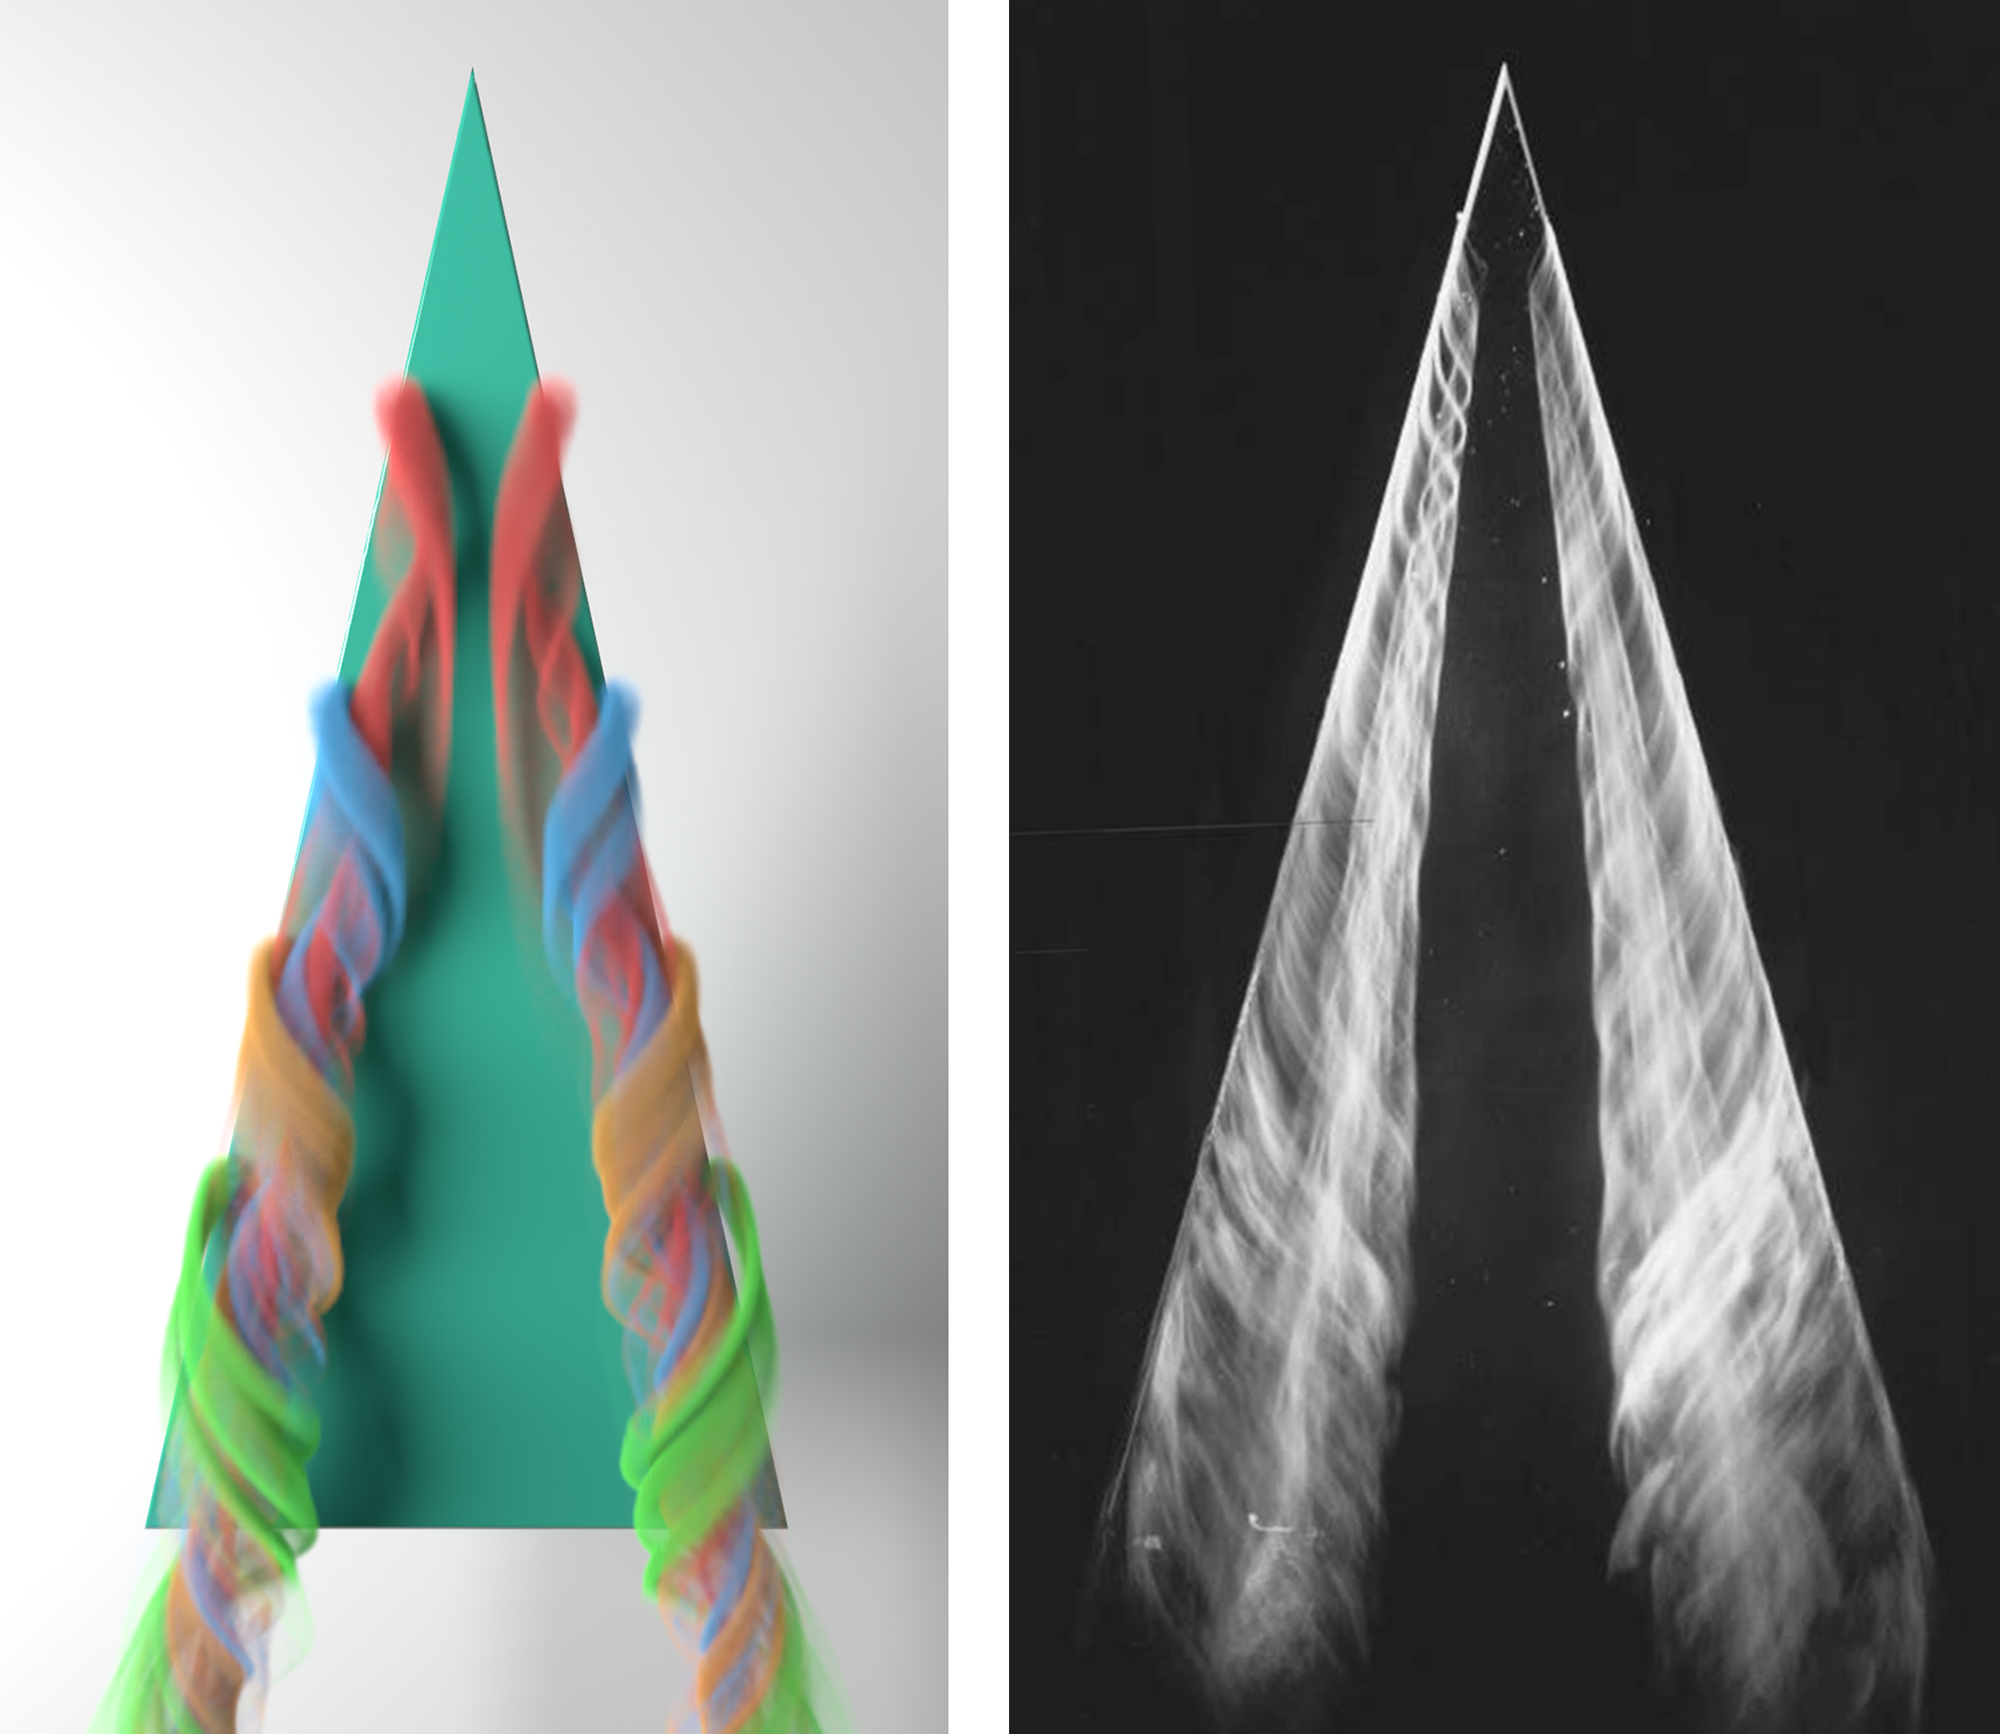
\includegraphics[width=0.99\columnwidth]{figures/comparison_delta_wing.png}
  \bicaption{三角翼仿真。通过我们的方法得到的薄板三角翼仿真结果 (左图) 与实际实验~\cite{Delery:2001} (右图) 的对比,展示出相同的前缘涡旋结构,表面我们的方法在薄结构边界层上的准确性。}{Delta-wing simulation. The airflow over a thin-shell delta-wing simulated with our hybrid coupling approach (left) matches experimental visualizations from~\cite{Delery:2001} (right), exhibiting the same spiral vortex structure near the leading edge of the wing and demonstrating the accuracy of our solver in capturing boundary layer flows around thin structures.}
  \label{img:comparison_delta_wing}
\end{figure}

% \paragraph{性能对比}
% As demonstrated in~\cite{Li-2020} and \cite{Chen-2021}, a kinetic solver has much higher computational performance than NS solvers, especially for turbulent flows with coupling where relatively small time steps are required.
% Since our new kinetic solver is built upon the same framework, we retain this competitive advantage even when their DI-IB boundary treatment is replaced by our hybrid method. However, because of our hybrid boundary treatment and new GPU optimizations discussed in Sec~\ref{sec:GPUopt}, we actually exceed their performance at all grid resolutions (using the same NVIDIA GeForce RTX 3090 GPU for fairness of comparisons) as shown in Fig.~\ref{fig:Performance}. Two factors are responsible for this improved computational efficiency: profiling the two codes shows, as expected, that our simplification of the collision operator via analytical LU decomposition~\cite{fei2018three} improves GPU occupancy, and that our hybrid coupling treatment with sample-based geometric approximations, despite being more accurate in practice, involve less computations with reduced penalty forces (less stiffness) than the original DI-IB method, thus allowing larger time steps for faster simulations. \vspace*{-1mm}

\begin{figure}[htb]
  \centering
    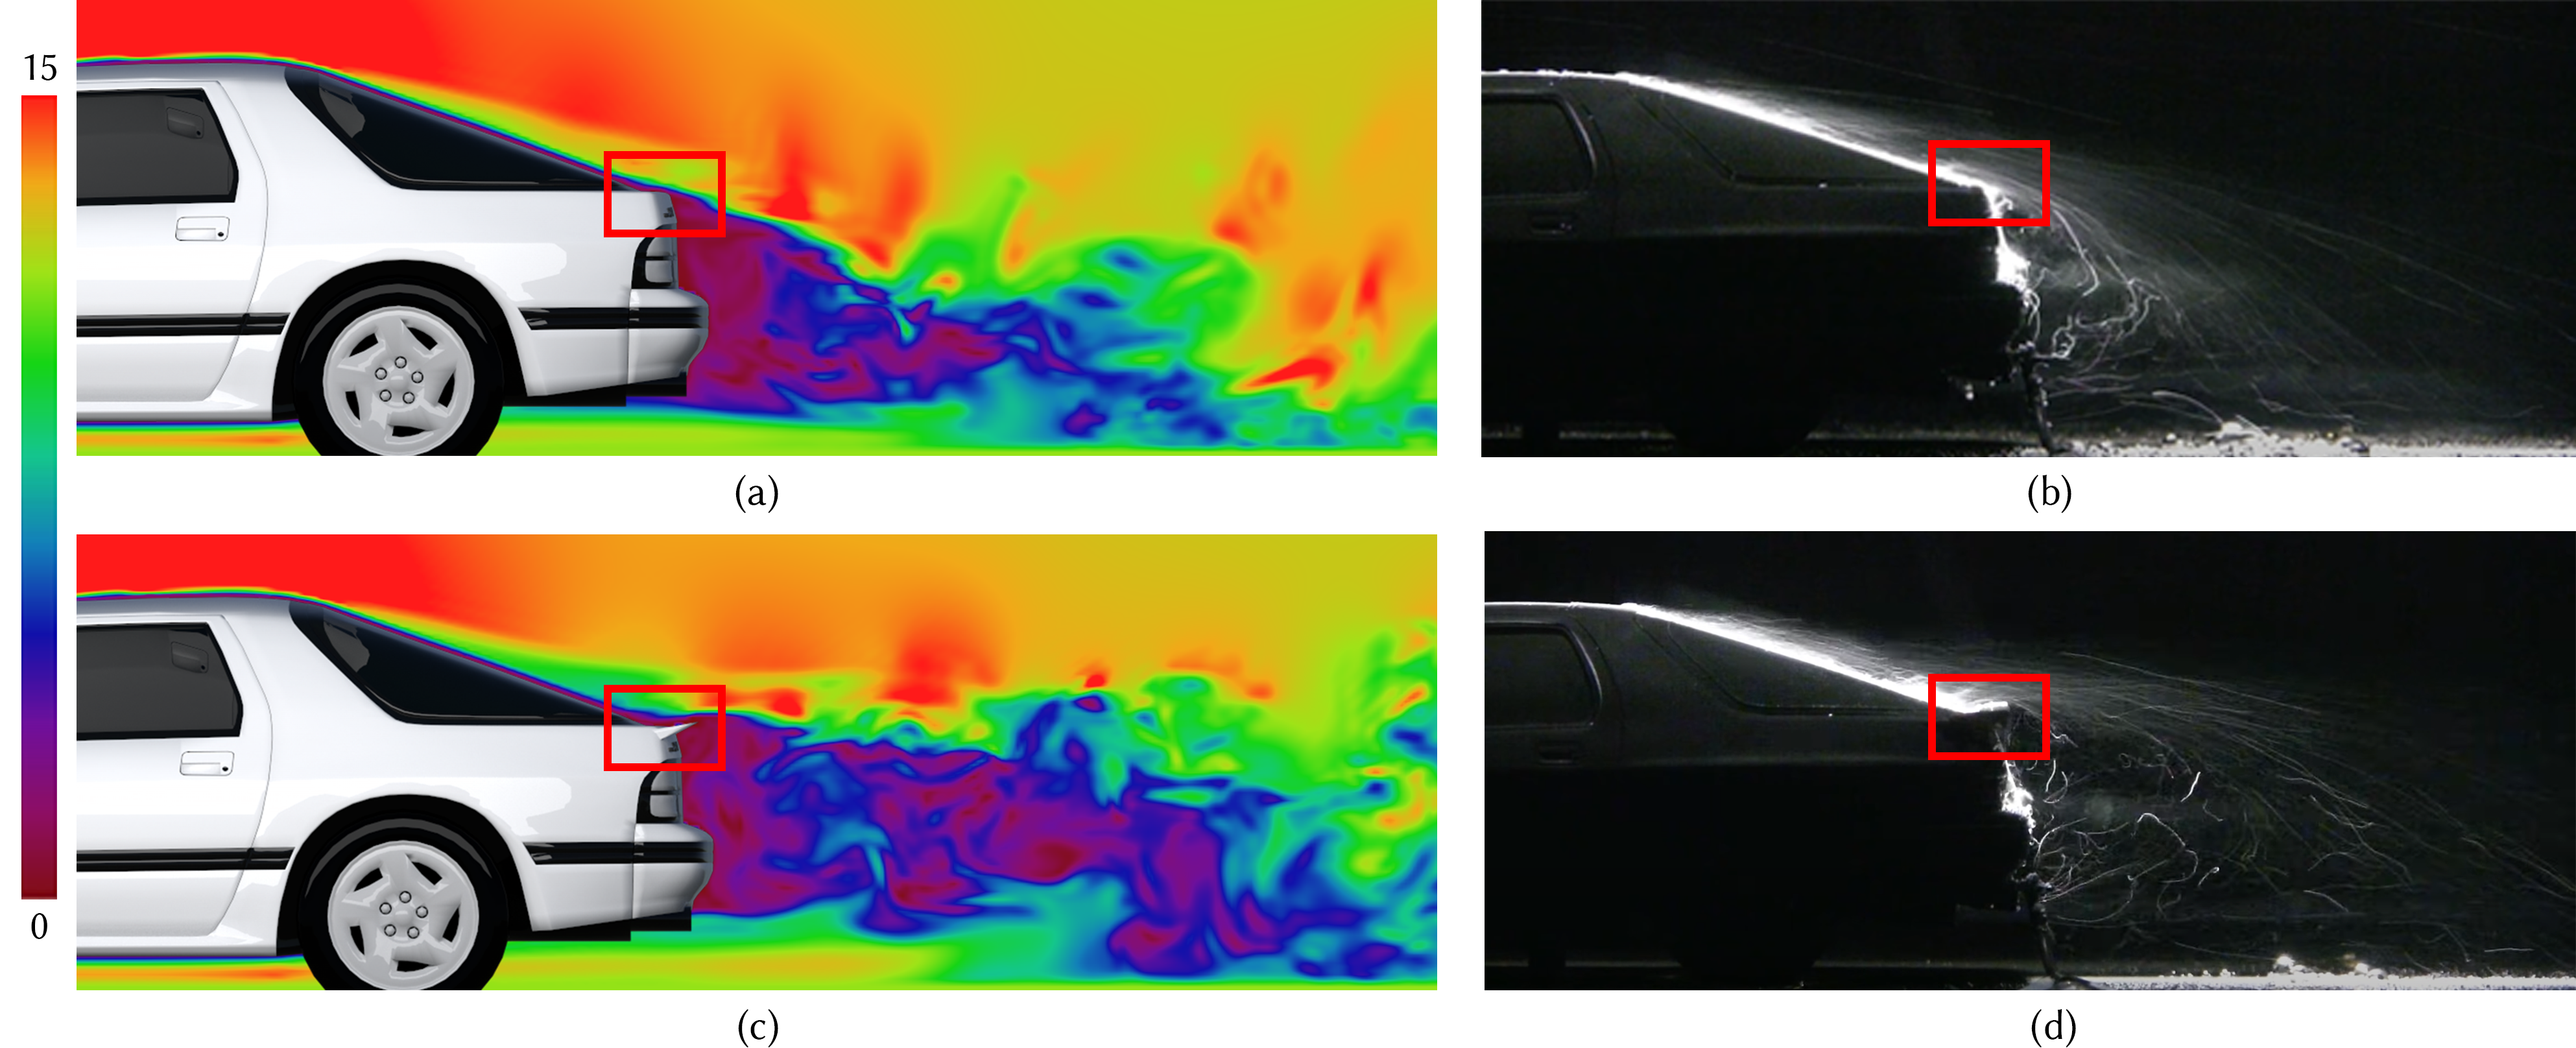
\includegraphics[width=0.99\columnwidth]{figures/comparsion_car_design.png}
  \bicaption{汽车的空气动力学设计。通过我们的方法对没有尾翼的汽车进行仿真 (a),其结果与一个相似的车辆模型在风洞可视化的结果匹配 (b)。之后添加一个小型的扰流板 (图中红色方框) 到汽车尾部之后,仿真中的尾流发生显著变化 (c),与带有扰流板的风洞测试相似 (d)。这展示出我们的方法可以快速、有效地为气动外形设计服务。图中的速度模值单位为$km/h$。图 (b) 与 (d) 的版权来自 Feltham~(\citeyear{youtube_2014})。}{Aerodynamic design of a car model. Simulating the airflow around a car model without a spoiler using our solver (a) matches the wind tunnel visualization for a similar car model (b); A small and thin spoiler (in red box) added on the back of the car model (c) changes the wake flow of the car model in our simulation quite significantly, in line with a wind-tunnel test of a car model with a spoiler (d) --- indicating that our solver offers an efficient, yet predictive tool of air flows for computational shape design. The velocity magnitude is measured in $km/h$. Image (b) and (d) courtesy of Feltham~(\citeyear{youtube_2014}).}
  \label{img:comparsion_car_design}
\end{figure}

\begin{figure}[htb]
  \centering
    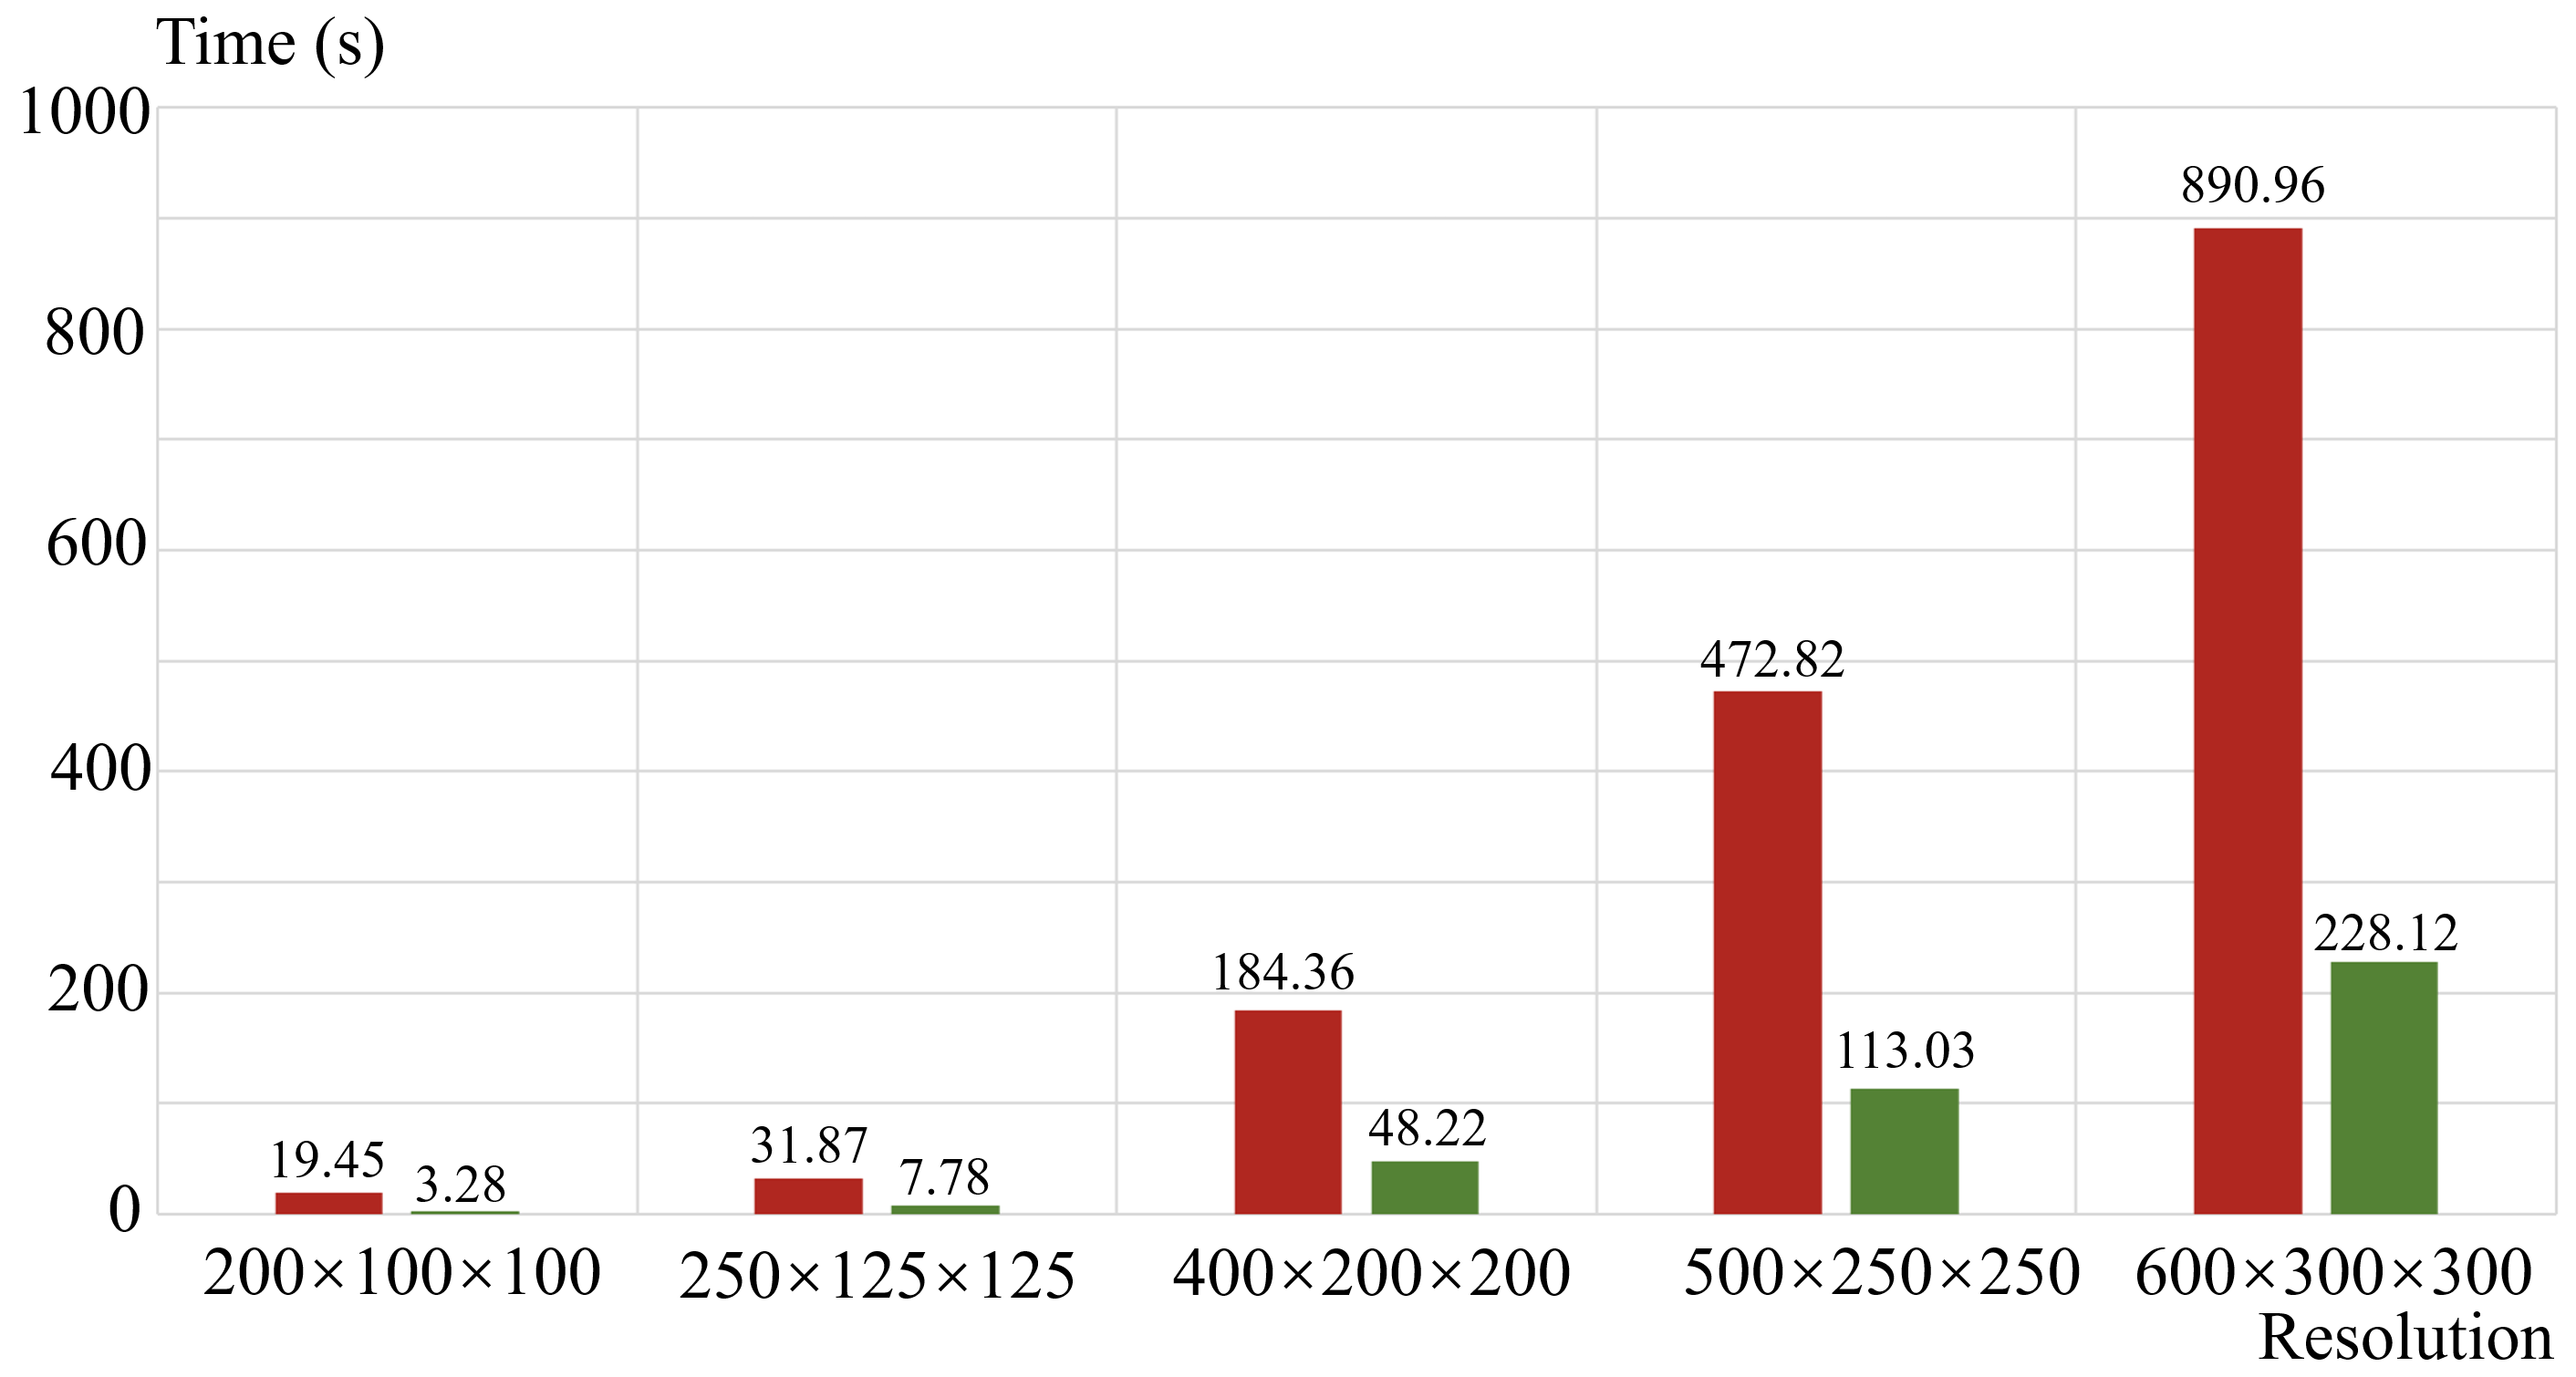
\includegraphics[width=0.93\columnwidth]{figures/performance.png}
  \bicaption{性能对比。我们将我们的方法 (绿色) 与Li等~(\citeyear{Li-2020})、Chen等~(\citeyear{Chen-2021}) 中的动力学求解方法 (红色) 进行比较,比较用例为图~\ref{img:comparsion_car_ib_ours} 中所示的汽车仿真,仿真时长为1秒。在同一张NVIDIA RTX 3090 GPU上得到的测试结果显示我们的方法在所有分辨率上都有显著的性能提升。}{Performance comparison. We compare the efficiency of the kinetic solver from~\cite{Li-2020,Chen-2021} (red) with our kinetic solver (green) based on one second of simulation of the car model shown in Fig.~\ref{img:comparsion_car_ib_ours} and both executed on a same NVIDIA RTX 3090 GPU, showing significant performance improvement for all grid resolutions.}
  \label{img:Performance}
\end{figure}

% \subsection{仿真结果}
% All simulations presented in this paper were conducted with our fluid simulator platform, on a workstation with a 14-core Intel Xeon E5-2690 CPU, 128 GB of memory and up to two NVIDIA RTX 3090 GPUs.
% We tested a number of different one-way and two-way examples and configurations with a wide range of geometric complexity to demonstrate that we can simulate fluid-solid coupling with both thick and thin solid structures, and for both laminar and turbulent flows. We also show a spectrum of results covering an interactive simulation as well as offline high-resolution large-scale simulations with complex solid structures to illustrate scalability. We discuss each example below (available in the \textit{supplementary video}).

\begin{figure}[htb]
  \centering
    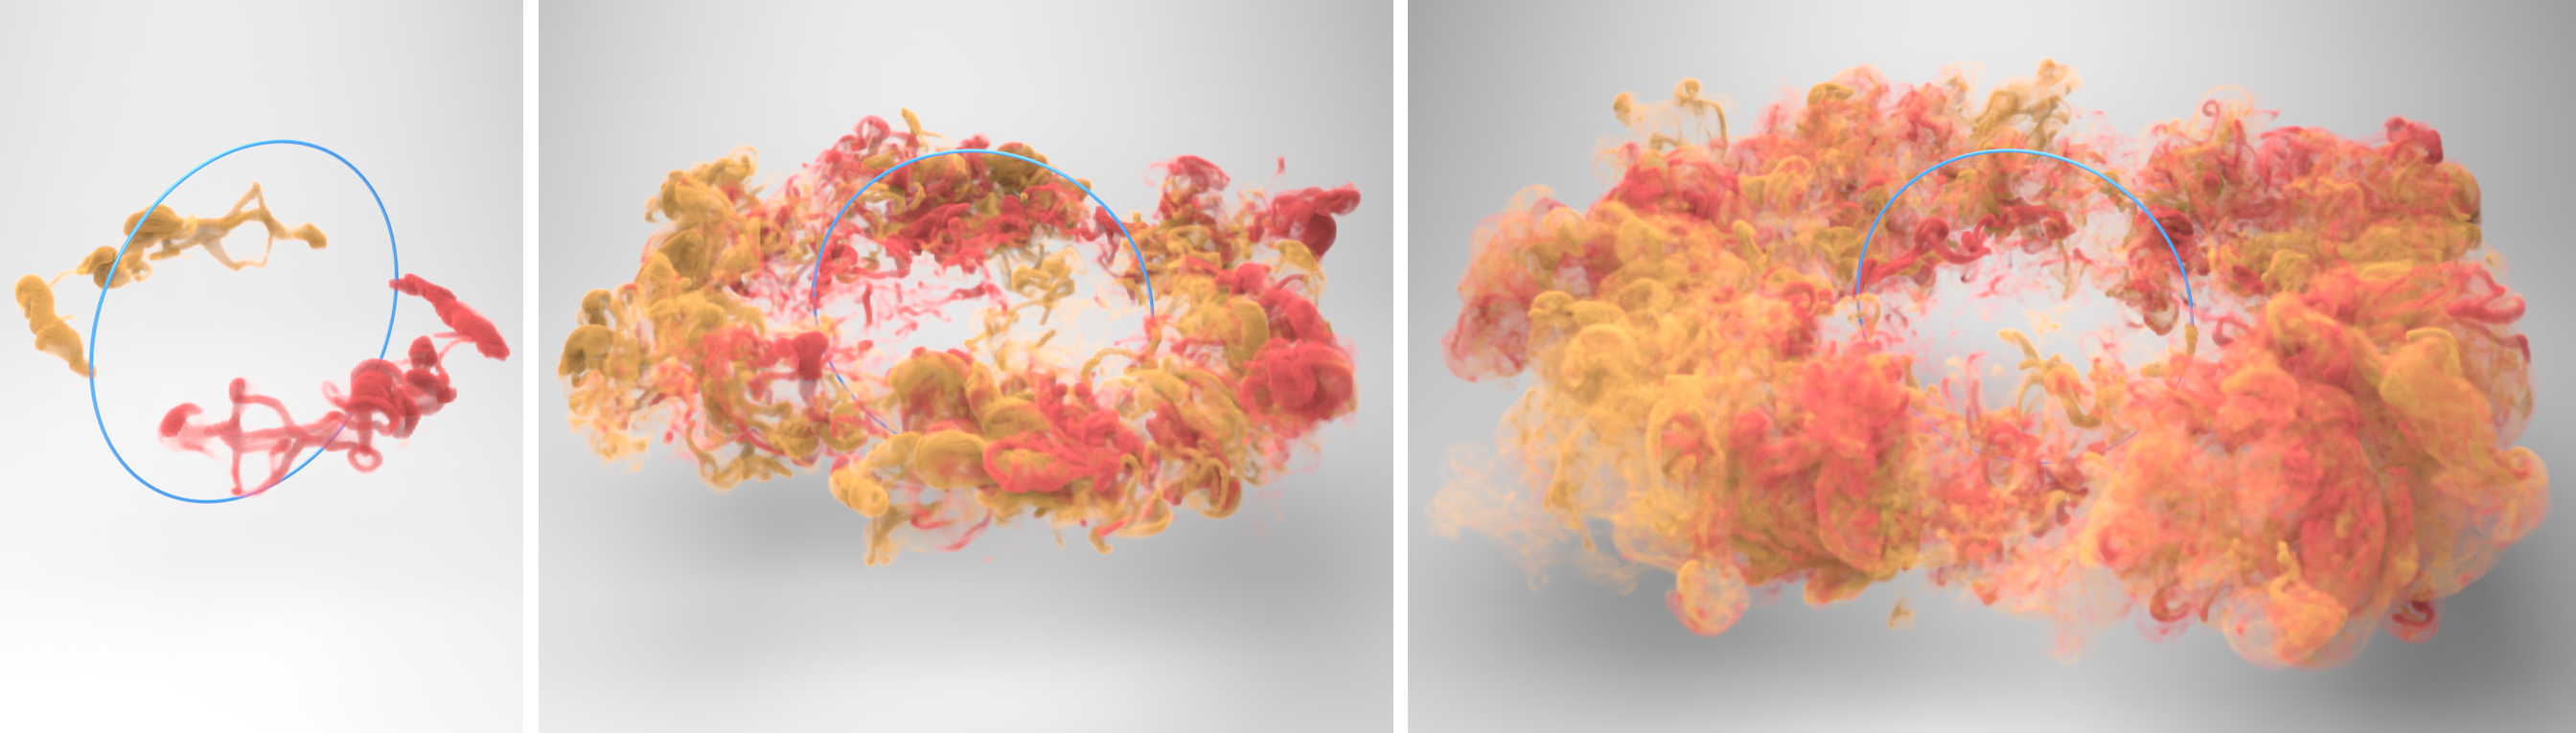
\includegraphics[width=0.99\columnwidth]{figures/result_rotating_torus.png}
  \bicaption{旋转的圆环。一个非常细的圆环沿着一个垂直轴旋转,在两侧发出黄色和橘色的烟雾,展示出圆环旋转所带出的湍流。}{Rotating ring. A very thin ring rotating along a vertical axis and emitting yellow and orange smoke particles is enough to create a turbulent wake as evidenced by the volutes of smoke resulting from the motion.}
  \label{img:result-rotating-torus}
\end{figure}

\begin{figure}[htb]
  \centering
    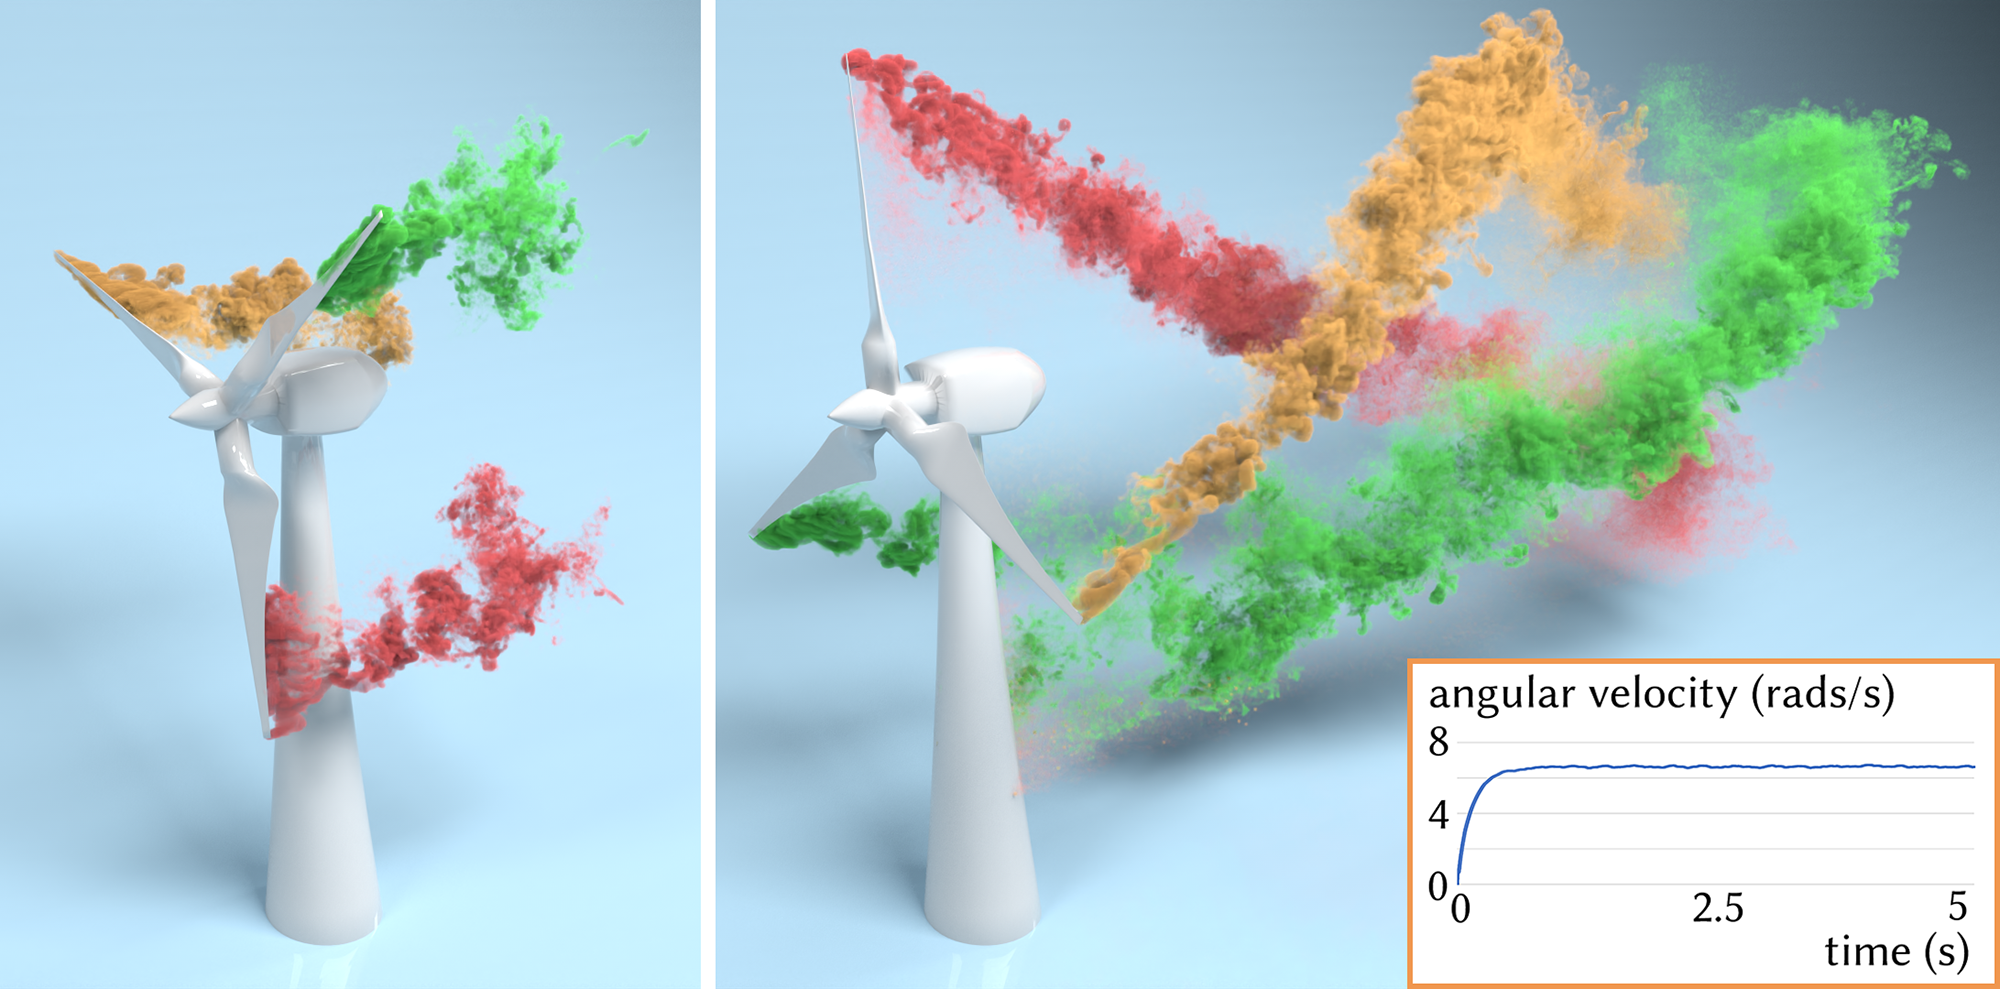
\includegraphics[width=0.99\columnwidth]{figures/result_wind_turbine.png}
  \bicaption{风力涡轮机的仿真。常速的风吹过一个有三个扇叶的风力涡轮机,驱动涡轮机旋转,并由扇叶上产生的烟雾对涡旋尾流结构进行可视化。这个双向的流固耦合结果考虑了轴上的摩擦力来限制了最大的角速度。扇叶角速度随时间的变化可见底部的小图。}{Turbine. A large turbine emitting colored smoke particles at the three propellers of its large blade is simulated with a constant incoming air flow making it turn, creating a spiral vortex trail. This two-way coupling example also involves friction on the axis of the turbine to limit its maximum angular velocity, resulting in a time-varying but converging curve of angular velocity of the turbine shown in the bottom inset.}
  \label{img:result-wind-turbine}
\end{figure}

\begin{figure}[htb]
  \centering
    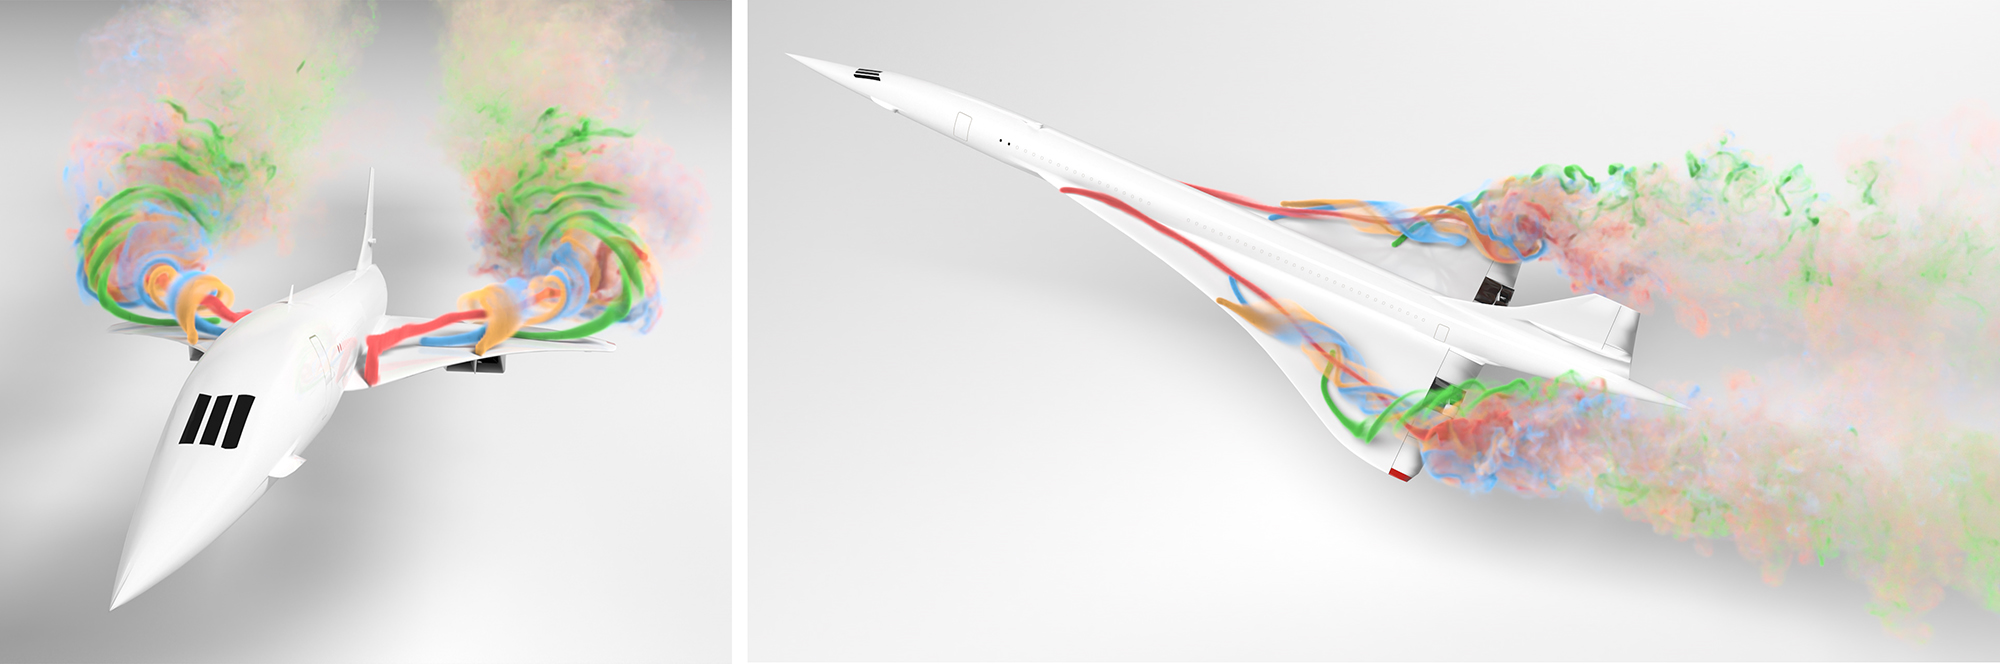
\includegraphics[width=0.99\columnwidth]{figures/teaser_concorde.jpg}
  \bicaption{飞机气动仿真。通过对协和客机翼面的气流仿真,我们展示出我们的方法可以同时处理含有薄板、细棒的薄物体以及厚物体的复杂几何。}{Aerodynamic simulation of an airplane. By simulting the flow over the wing of the Concorde airplane, we demonstrate that our method can handle complex solids containing thin shells, rods and thick objects.}
  \label{img:teaser_concorde}
\end{figure}

% \vspace*{-1mm}
% \paragraph{Coupling with thin shells}
% We first simulate a simple thin shell in the shape of a cylinder rotating at a constant speed, and thus generating a shear flow, see Fig.~\ref{fig:result-tube}; this setup computed at low Reynolds number (high viscosity) exhibits a very different behavior from its high Reynolds number (low viscosity) counterpart, as expected.
% A case where multiple thin shells are piling up is also tested, see Fig.~\ref{fig:result-thin-shell-sub-grid}, where the plates are first well separated, before getting stacked up. Here, our sub-grid approximation produces plausible coupling results, with a seamless transition between separate plates early on and an airtight block of plates by the end of the animation: our method degrades gracefully in the presence of obstacles that it cannot be resolved by the grid. A two-way coupling example in Fig.~\ref{fig:result-blowing-leaves} shows dried-up leaves (each far thinner than a grid cell size) being blown by an upward gust of wind. As expected, the dead leaves are lifted up by the air flow, and fall back slowly on the ground while being rotated by the surrounding air.

% \vspace*{-1mm}
% \paragraph{Coupling with thin rods}
% We also show that our solver can handle thin rods, first with a simple example where a thin ring-like object rotates with a constant speed in the air. Our boundary treatment method generates a reasonable turbulent wake flow, see Fig.~\ref{fig:result-rotating-torus}.
% When several rods are grouped together, our sub-grid approximation still creates visually plausible coupling results as demonstrated in Fig.~\ref{fig:result-thin-rod-sub-grid}; note the increased amount of turbulent flows near the solid boundary as well as in the wake due to the addition of bristles.

% \vspace*{-1mm}
% \paragraph{Coupling with complex solid}
% A more complicated, yet very common case is when both thick and thin structures form a complex solid shape that interacts with a fluid.
% Our hybrid boundary treatment method is an efficient and unified approach to supporting such cases. Indeed,
% Fig.~\ref{fig:result-wind-turbine} shows the two-way coupling simulation of a three-blade wind turbine where the air flow blows through the turbine to drive its rotating motion, and in turn, the air flow gets affected by the motion. Additionally,
% Fig.~\ref{fig:teaser_concorde} shows a simulation of the Concorde airplane flying in the air with an angle of attack of $20^\circ$; for such a complex shape and for a reasonable grid size, many of the plane's parts (in particular near the wings) are thin structures. In both cases, the results are consistent with expectations.

\begin{figure}[htb]
  \centering
    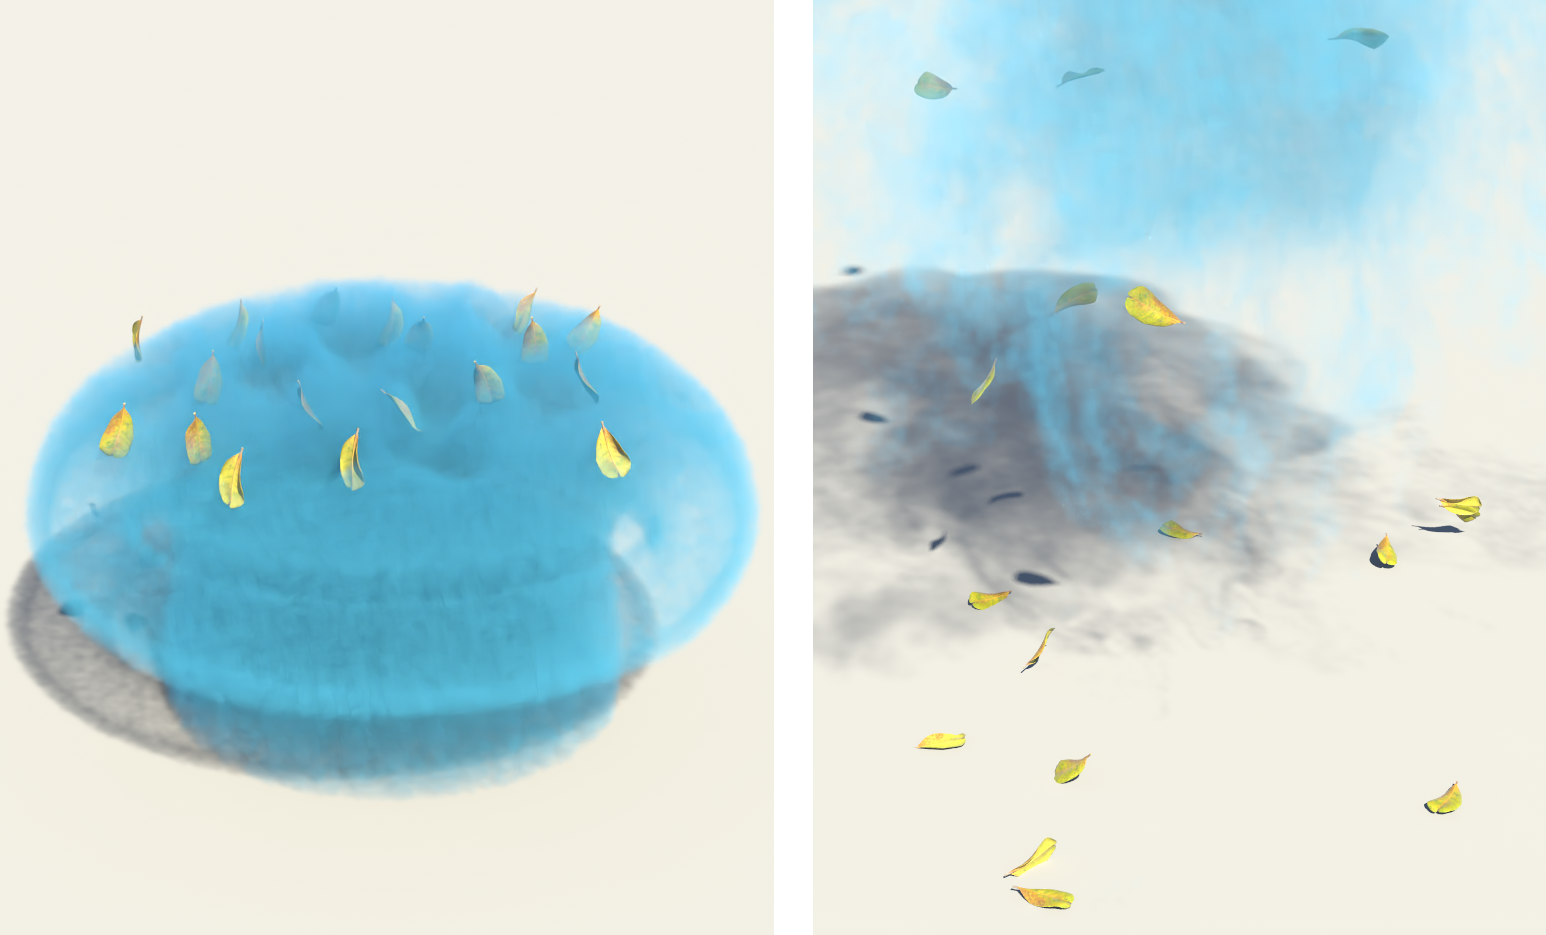
\includegraphics[width=0.99\columnwidth]{figures/result_blowing_leaves.png}
  \bicaption{风吹叶子的仿真。在这个双向流固耦合结果中,一阵风从地面吹起将树叶吹向空中。}{Wind blowing leaves. In this two-way coupling example, a puff of wind from the ground drives a bunch of dried-up leaves up in the air.}
  \label{img:result-blowing-leaves}
\end{figure}

% \vspace*{-1mm}
% \paragraph{Fast simulation for interactive design}
% Our fluid-solid coupling simulator is particularly efficient given its high level of parallelism, which allows for interactive testing of product design even with a single GPU. As an example, an interactive simulation conducted with a $200\!\times\!200\!\times\!200$ grid resolution for a fast rotating blade is performed in Fig.~\ref{fig:result-design}, where a cross-sectional magnitude plot of the velocity field of the surrounding air is displayed.
% One frame corresponding to an animation of 1/100 s. is computed in less than $0.4$ second including the data read-back and visualization time (cross-section visualization is currently done on CPU), meaning that a preliminary design of the blade can be quickly evaluated, e.g., for turbulence reduction by optimizing the geometric shape. Our supplementary video contains a recording of the whole user interaction on our simulation platform for this example, captured in real time.

\begin{figure}[htb]
  \centering
    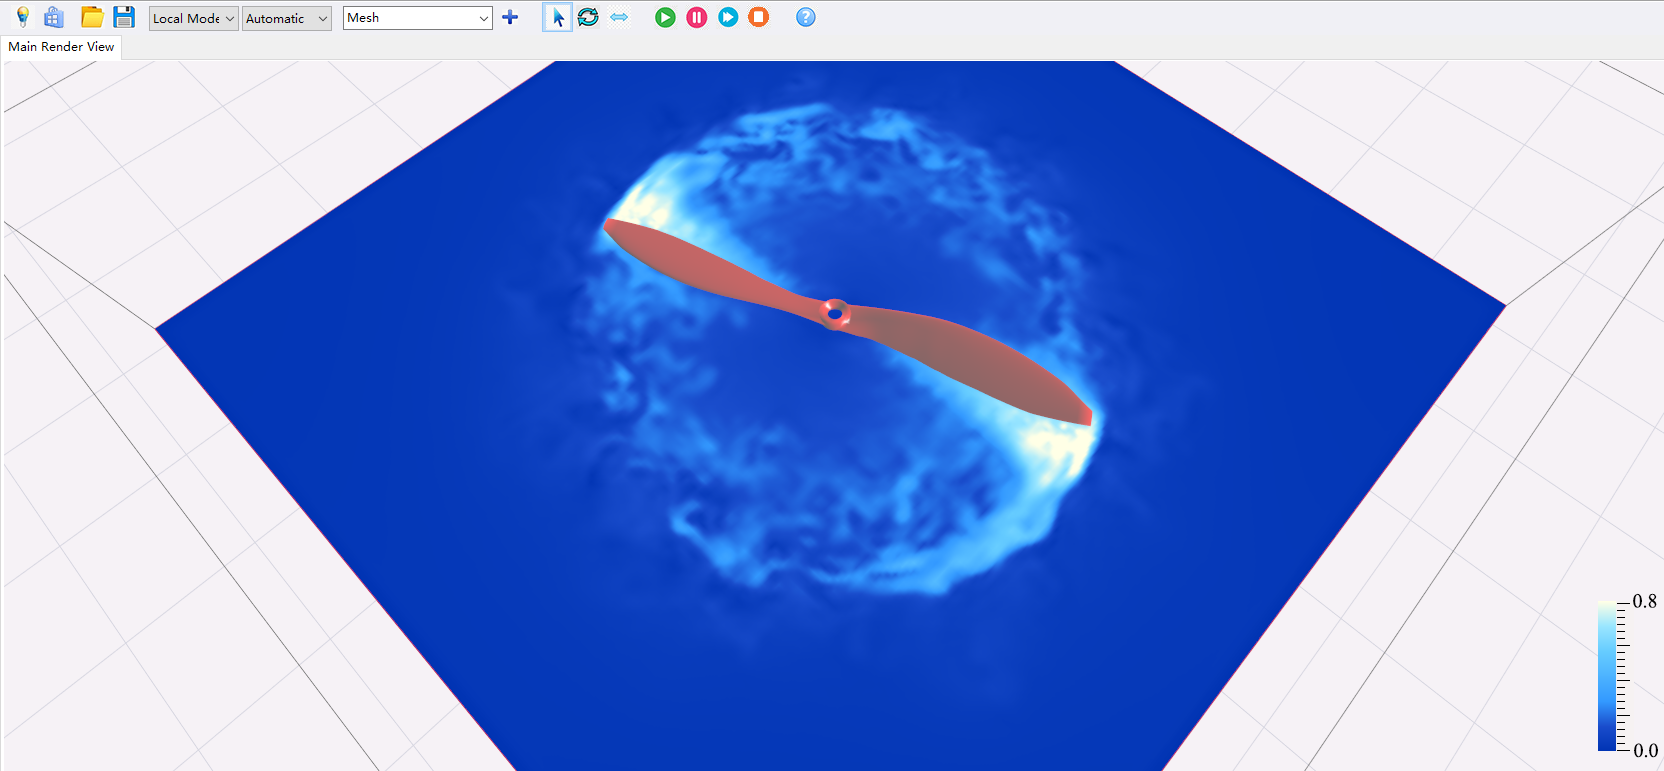
\includegraphics[width=0.99\columnwidth]{figures/result_design.png}
  \bicaption{快速交互设计。我们通过GUI操作模拟系统,来快速生成仿真结果。图中示例为一个快速旋转的旋翼,我们可以通过可视化即时的看到尾流情况。这样的快速交互式仿真可以用来辅助产品设计与验证。}{Fast simulation for interactive design. We operated our GUI-based simulation system to produce a quick preliminary result of a fast rotating rotor-blade where turbulent wake flows can be observed interactively, which is very useful for efficient product design and verification.}
  \label{img:result-design}
\end{figure}

\begin{figure}[htb]
  \centering
    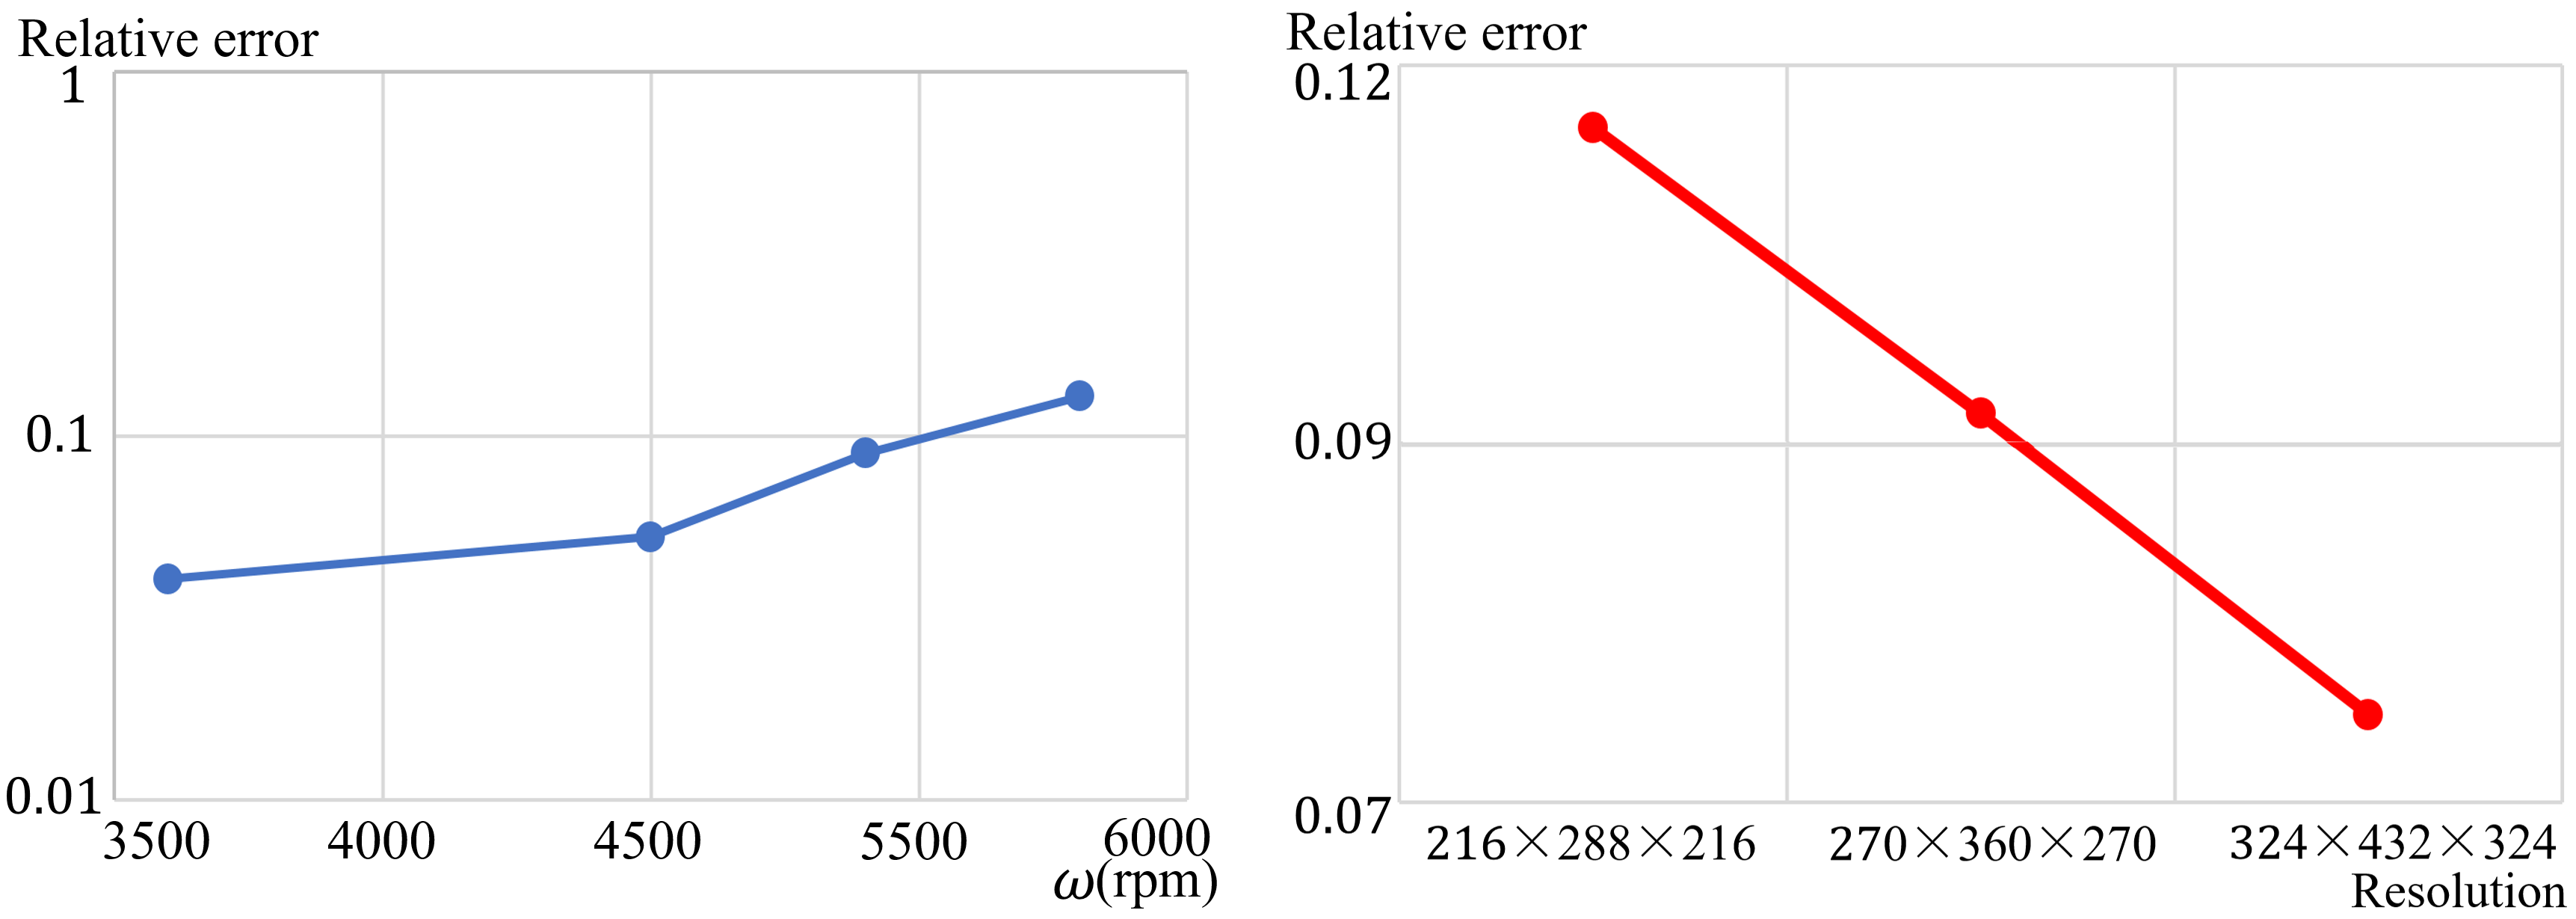
\includegraphics[width=0.99\columnwidth]{figures/DJI_compare.png}
  \bicaption{推力的验证。我们通过旋翼旋转的气动仿真来测试旋翼的推力。我们在$288\!\times\!324\!\times\!288$分辨率下测试不同转速的误差结果见左图。右图为固定3600 rpm转速时,相对误差的收敛情况。注意我们采用的分辨率并不是非常高,所以结果的精度依然有提升空间。}{Thrust evaluation. From the simulation of the coupling between a rotating drone blade and the surrounding air, we can compute the estimated thrust values at different rotation speeds with a grid resolution of $288\!\times\!324\!\times\!288$ (left). The relative errors of our thrust value at 3600 rpm w.r.t. experimental measurements as the grid resolution increases (right) indicates convergence of our solver. Note that the tested grid resolutions are not very high, and more accurate results are expected for higher grid resolutions.}
  \label{img:DJI_thrust_compare}
\end{figure}

% \paragraph{High-resolution simulations}
% Finally, we simulate a high-resolution large-scale scenario to demonstrate the scalability of our approach, using this time two GPUs.
% Fig.~\ref{fig:result-city} shows a mass of smoke particles passing through a neighborhood of a high-rise, high-density city, where the buildings containing thin and sharp structures affect the air flow. For this very large-scale example with fine turbulence details, 5 seconds of animation took only around 1.5 hours to compute; as discussed in detail in~\cite{Li-2020}, such an efficiency for this level of accuracy is currently out of reach for NS-based solvers even with multi-GPU accelerations: their pressure projection and implicit viscosity handling require accurate matrix solves that are too time consuming if realistic vortical structures are desired.

% \section{方法的局限性}
% Despite its excellent numerical results and increased generality, our method still suffers from limitations.
% First, due to our sample-based geometric representation, the approximate bounce-back scheme may have undesired behavior at extremely sharp corners, for example, at the tip of a delta wing, since the projection achieved via the nearest available sample may not be accurate.
% Increasing sample size or using adaptive sampling can improve the accuracy, but at a cost of more memory usage.
% For visual applications, however, the resulting animations are not particularly different, so this issue mostly matters for the rapid testing of product design.
% Second, our total force and torque applied to the solid resulting from our two-way coupling approach inherit the typical limitation of a staircase approximation of the solid boundary on grid: for coarse grids, our proposed sub-grid approximation cannot faithfully reflect the true geometry, affecting the accuracy of the force and torque on solid.  Finally, an efficient sampling method that can adjust to a deforming geometry is currently needed.

% \section{总结}
% In this paper, we proposed a hybrid coupling treatment for kinetic solvers that enables robust, fast and plausible handling of a large variety of obstacle shapes including both thick and thin structures. Our approach leverages the complementary advantages of the bounce-back scheme and the sharp-interface immersed boundary method by introducing a novel unified approach: it consists of a double-sided bounce-back treatment followed by a one-sided velocity correction, together with a hybrid boundary force and torque calculation to enable two-way coupling.
% Efficient geometric approximations based on boundary point-samples (along with their parallel implementations on GPU) were proposed to improve computational performance, and further improvements in the GPU implementation of existing LBM solvers were also offered.
% The resulting simulator was shown to exceed the accuracy of existing state-of-the-art solvers, to further improve on their efficiency, and to capture the correct physical behavior of complex fluid-solid interactions even for very turbulent flows.
% A wide range of simulation results with different types of immersed boundary shapes were demonstrated, followed by comparisons to other coupling methods as well as physical experiments to show the potential applicability of our method in both efficient visual production and fast computational design. This capacity to rival both CG-based and CFD-based fluid methods in efficiency and accuracy is particularly promising, and we hope it will lead to a variety of follow-up works in both communities.